\documentclass[12pt,a4paper]{article}

\usepackage[a4paper, margin=1in]{geometry}
\usepackage[utf8]{inputenc}
\usepackage{graphicx}
\usepackage{booktabs}
\usepackage{array}
\usepackage{amsmath}
\usepackage{hyperref}
\usepackage{caption}
\usepackage{subcaption}
\usepackage{float}
\usepackage{parskip}
\usepackage{titlesec}
\usepackage{xcolor}
\usepackage{microtype}

\hypersetup{colorlinks=true,linkcolor=blue!60!black,urlcolor=blue!60!black,citecolor=blue!60!black}
\titleformat{\section}{\large\bfseries}{}{0em}{\thesection\quad}
\titleformat{\subsection}{\normalsize\bfseries}{}{0em}{\thesubsection\quad}
\graphicspath{{./outputs/}}

% All numbers auto-generated by main.py via generate_report_text.py
% Auto-generated by generate_report_text.py - do not edit manually.
% Re-run python main.py to update all values.

% -- KNN
\newcommand{\knnBoWAcc}{53.12\%}
\newcommand{\knnBertAcc}{88.06\%}
\newcommand{\knnJumpPP}{35}

% -- Logistic Regression
\newcommand{\lrBoWAcc}{85.94\%}
\newcommand{\lrTfidfAcc}{88.88\%}
\newcommand{\lrSvdAcc}{86.12\%}
\newcommand{\lrBertAcc}{88.62\%}
\newcommand{\lrBertPcaAcc}{89.06\%}
\newcommand{\lrBertImprove}{88.62\% $\to$ 89.06\%}
\newcommand{\lrTfidfDrop}{88.88\% $\to$ 86.12\%}

% -- Linear SVM
\newcommand{\lsvmTfidfAcc}{88.62\%}
\newcommand{\lsvmSvdAcc}{86.00\%}
\newcommand{\lsvmTfidfDrop}{88.62\% $\to$ 86.00\%}
\newcommand{\lsvmBertAcc}{87.38\%}
\newcommand{\lsvmPcaAcc}{88.94\%}

% -- RBF SVM
\newcommand{\rbfBertPcaAcc}{90.19\%}
\newcommand{\rbfBertAcc}{89.19\%}

% -- Best overall
\newcommand{\bestAcc}{90.19\%}
\newcommand{\bestFscore}{90.09\%}
\newcommand{\bestModel}{RBF SVM}
\newcommand{\bestFeat}{Reduced DistilBERT (PCA)}

% -- Variance retention
\newcommand{\bertPcaVar}{85.89\%}
\newcommand{\tfidfSvdVar}{16.19\%}
\newcommand{\glovePcaVar}{100.00\%}

% -- KMeans
\newcommand{\kmBowNmi}{0.0452}
\newcommand{\kmBowAri}{0.0142}
\newcommand{\kmTfidfNmi}{0.2411}
\newcommand{\kmBertNmi}{0.5589}
\newcommand{\kmBertAri}{0.5727}
\newcommand{\kmGloveNmi}{0.4504}
\newcommand{\kmGloveAri}{0.3840}

% -- GloVe
\newcommand{\gloveBestAcc}{87.75\%}
\newcommand{\gloveRbfAcc}{87.75\%}

% -- Confusion matrix
\newcommand{\cmSportsCorrect}{405}
\newcommand{\cmSportsTotal}{408}
\newcommand{\cmBizToSci}{48}
\newcommand{\cmSciToBiz}{26}

% -- Dataset
\newcommand{\nSamples}{8{,}000}
\newcommand{\nClasses}{4}
\newcommand{\nTrain}{6{,}400}
\newcommand{\nTest}{1{,}600}
\newcommand{\vocabSize}{5{,}000}


\begin{document}

\begin{center}
    {\LARGE\bfseries Statistical Machine Learning Course Project}\\[0.4em]
    {\large Text Classification: Sparse Features vs Static and Contextual Embeddings}\\[1em]
    {\normalsize Sharma Dhruv M Ram \quad|\quad Roll No: BA2025044}\\[0.2em]
    {\normalsize International Institute of Information Technology (IIIT), Bangalore}\\[0.2em]
    {\normalsize April 2026}
\end{center}
\hrule\vspace{1em}

\section{Introduction and Dataset Used}

The primary objective of this project is to explore and compare the efficacy of classical
statistical machine learning models when applied to three fundamentally different text
representation paradigms. We contrast traditional sparse feature extraction
(Bag-of-Words and TF-IDF), static dense word embeddings (GloVe), and modern contextual
embeddings from a pre-trained language model (DistilBERT). The project strictly utilises
classical models like Logistic Regression, Linear SVM, RBF SVM, KNN, and KMeans, to
evaluate these feature spaces, treating DistilBERT and GloVe purely as feature extractors
with no fine-tuning performed.

This three-way comparison is deliberate. It allows us to isolate precisely \textit{what}
drives performance gains: is it simply using dense vectors instead of sparse ones, or
does the contextual nature of DistilBERT provide additional discriminative power beyond
what static word embeddings can offer?

\section{Dataset Description and EDA}

The models were trained and evaluated on the \textbf{AG News} dataset, accessed via the
Hugging Face \texttt{datasets} library. Exactly \nSamples{} samples were selected using
a fixed random seed (\texttt{seed=42}) to ensure reproducibility.

\subsection{Class Distribution}
As shown in Figure~\ref{fig:eda}, the dataset is near-uniformly distributed across
\nClasses{} target classes: \textit{World}, \textit{Sports}, \textit{Business}, and
\textit{Sci/Tech}, each containing approximately 2,000 samples. This balance eliminates
class imbalance as a confounding factor in accuracy measurements.

\subsection{Token Length Distribution}
Article lengths follow a roughly normal distribution peaking at 40--45 words per article,
with very few outliers exceeding 100 tokens.

\subsection{Top Terms and Discriminative Vocabulary}
The most frequent unigrams after stop-word removal are dominated by newswire markers.
Figure~\ref{fig:wordclouds} visualises the \textit{discriminative} vocabulary per class
extracted from Logistic Regression coefficients.

\begin{figure}[H]
    \centering
    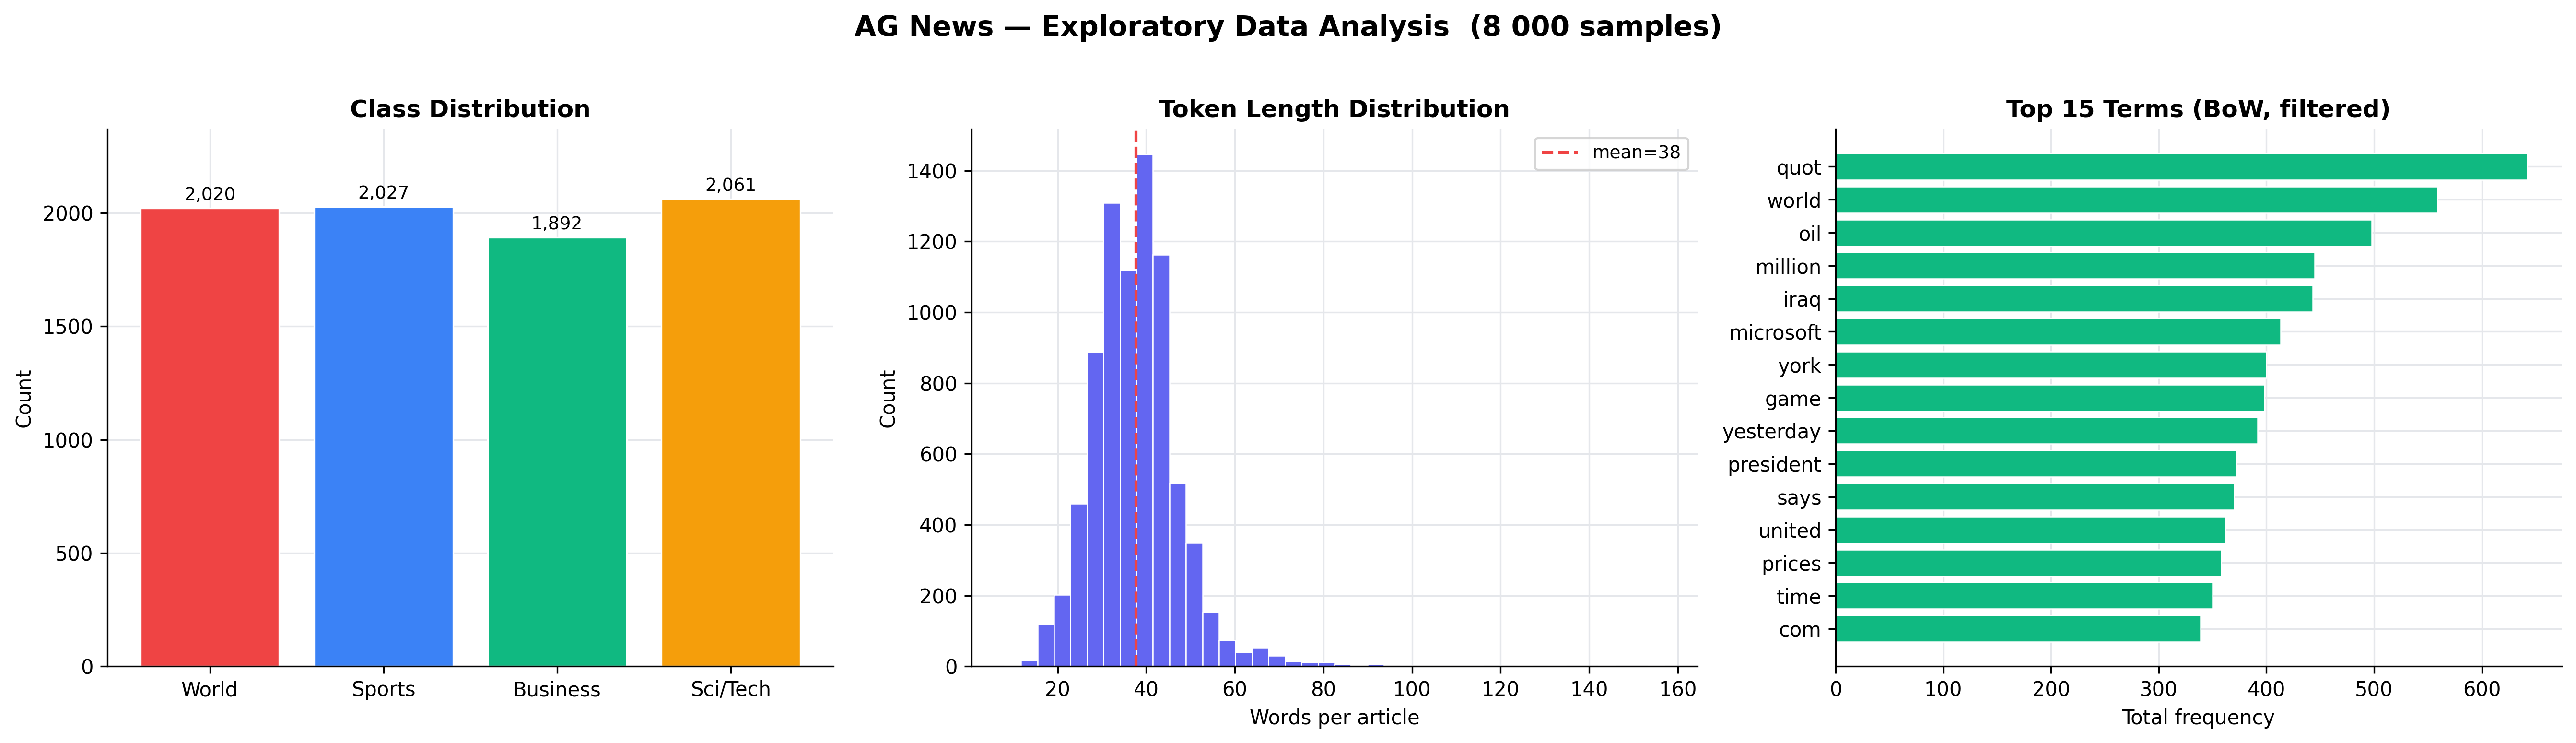
\includegraphics[width=\textwidth]{01_eda_plots.png}
    \caption{EDA overview: class distribution (left), token length histogram (centre),
             and top-15 filtered unigrams after stop-word removal (right).}
    \label{fig:eda}
\end{figure}

\begin{figure}[H]
    \centering
    
\includegraphics[width=\textwidth]{02_wordclouds_lr_features.png}
    \caption{Discriminative vocabulary per class (word size $\propto$ LR coefficient).
             Sports vocabulary is highly domain-specific; Business and Sci/Tech share
             technological vocabulary, foreshadowing their confusion in classification.}
    \label{fig:wordclouds}
\end{figure}

\section{Methodology}

\subsection{Part A: Sparse Features}
Two representations were generated after standard preprocessing:
\begin{itemize}
    \item \textbf{Unigram Bag-of-Words (BoW):} Raw term frequencies, vocabulary pruned
          to \vocabSize{} features, minimum document frequency of 2.
    \item \textbf{Unigram + Bigram TF-IDF:} Word and word-pair features with
          log-normalised TF (\texttt{sublinear\_tf=True}), limited to \vocabSize{} features.
\end{itemize}

\subsection{Part B: Static Dense Embeddings (GloVe, Bonus)}
100-dimensional GloVe vectors (Wikipedia 2014 + Gigaword 5, 6B tokens) loaded via
gensim. Each document represented as the arithmetic mean of known GloVe word vectors,
cached as a \texttt{.npy} file. GloVe acts as a \textit{static semantic} intermediate:
unlike BoW it encodes word-level semantic similarity, but unlike DistilBERT it lacks
\textit{contextual disambiguation}.

\subsection{Part C: Contextual Embeddings (DistilBERT)}
The frozen \texttt{distilbert-base-uncased} model was used strictly as a feature
extractor. The \texttt{[CLS]} token from the final hidden state yielded a dense
768-dimensional vector per article, computed once on GPU (Kaggle) and cached.

\subsection{Part D: Models}
\begin{itemize}
    \item Logistic Regression (\texttt{max\_iter=1000})
    \item Linear SVM
    \item RBF SVM
    \item K-Nearest Neighbours ($K=5$)
    \item KMeans ($K=4$, unsupervised baseline)
\end{itemize}

\subsection{Part E: Dimensionality Reduction}
Feature spaces were compressed to 100 dimensions.
\begin{itemize}
    \item \textbf{Truncated SVD} on TF-IDF: retains only \textbf{\tfidfSvdVar};
          the sparse space is nearly isotropic.
    \item \textbf{PCA} on DistilBERT: retains \textbf{\bertPcaVar}; strong
          structure concentrated in a small subspace.
    \item \textbf{PCA} on GloVe: retains \textbf{\glovePcaVar} (compression check).
\end{itemize}

\begin{figure}[H]
    \centering
    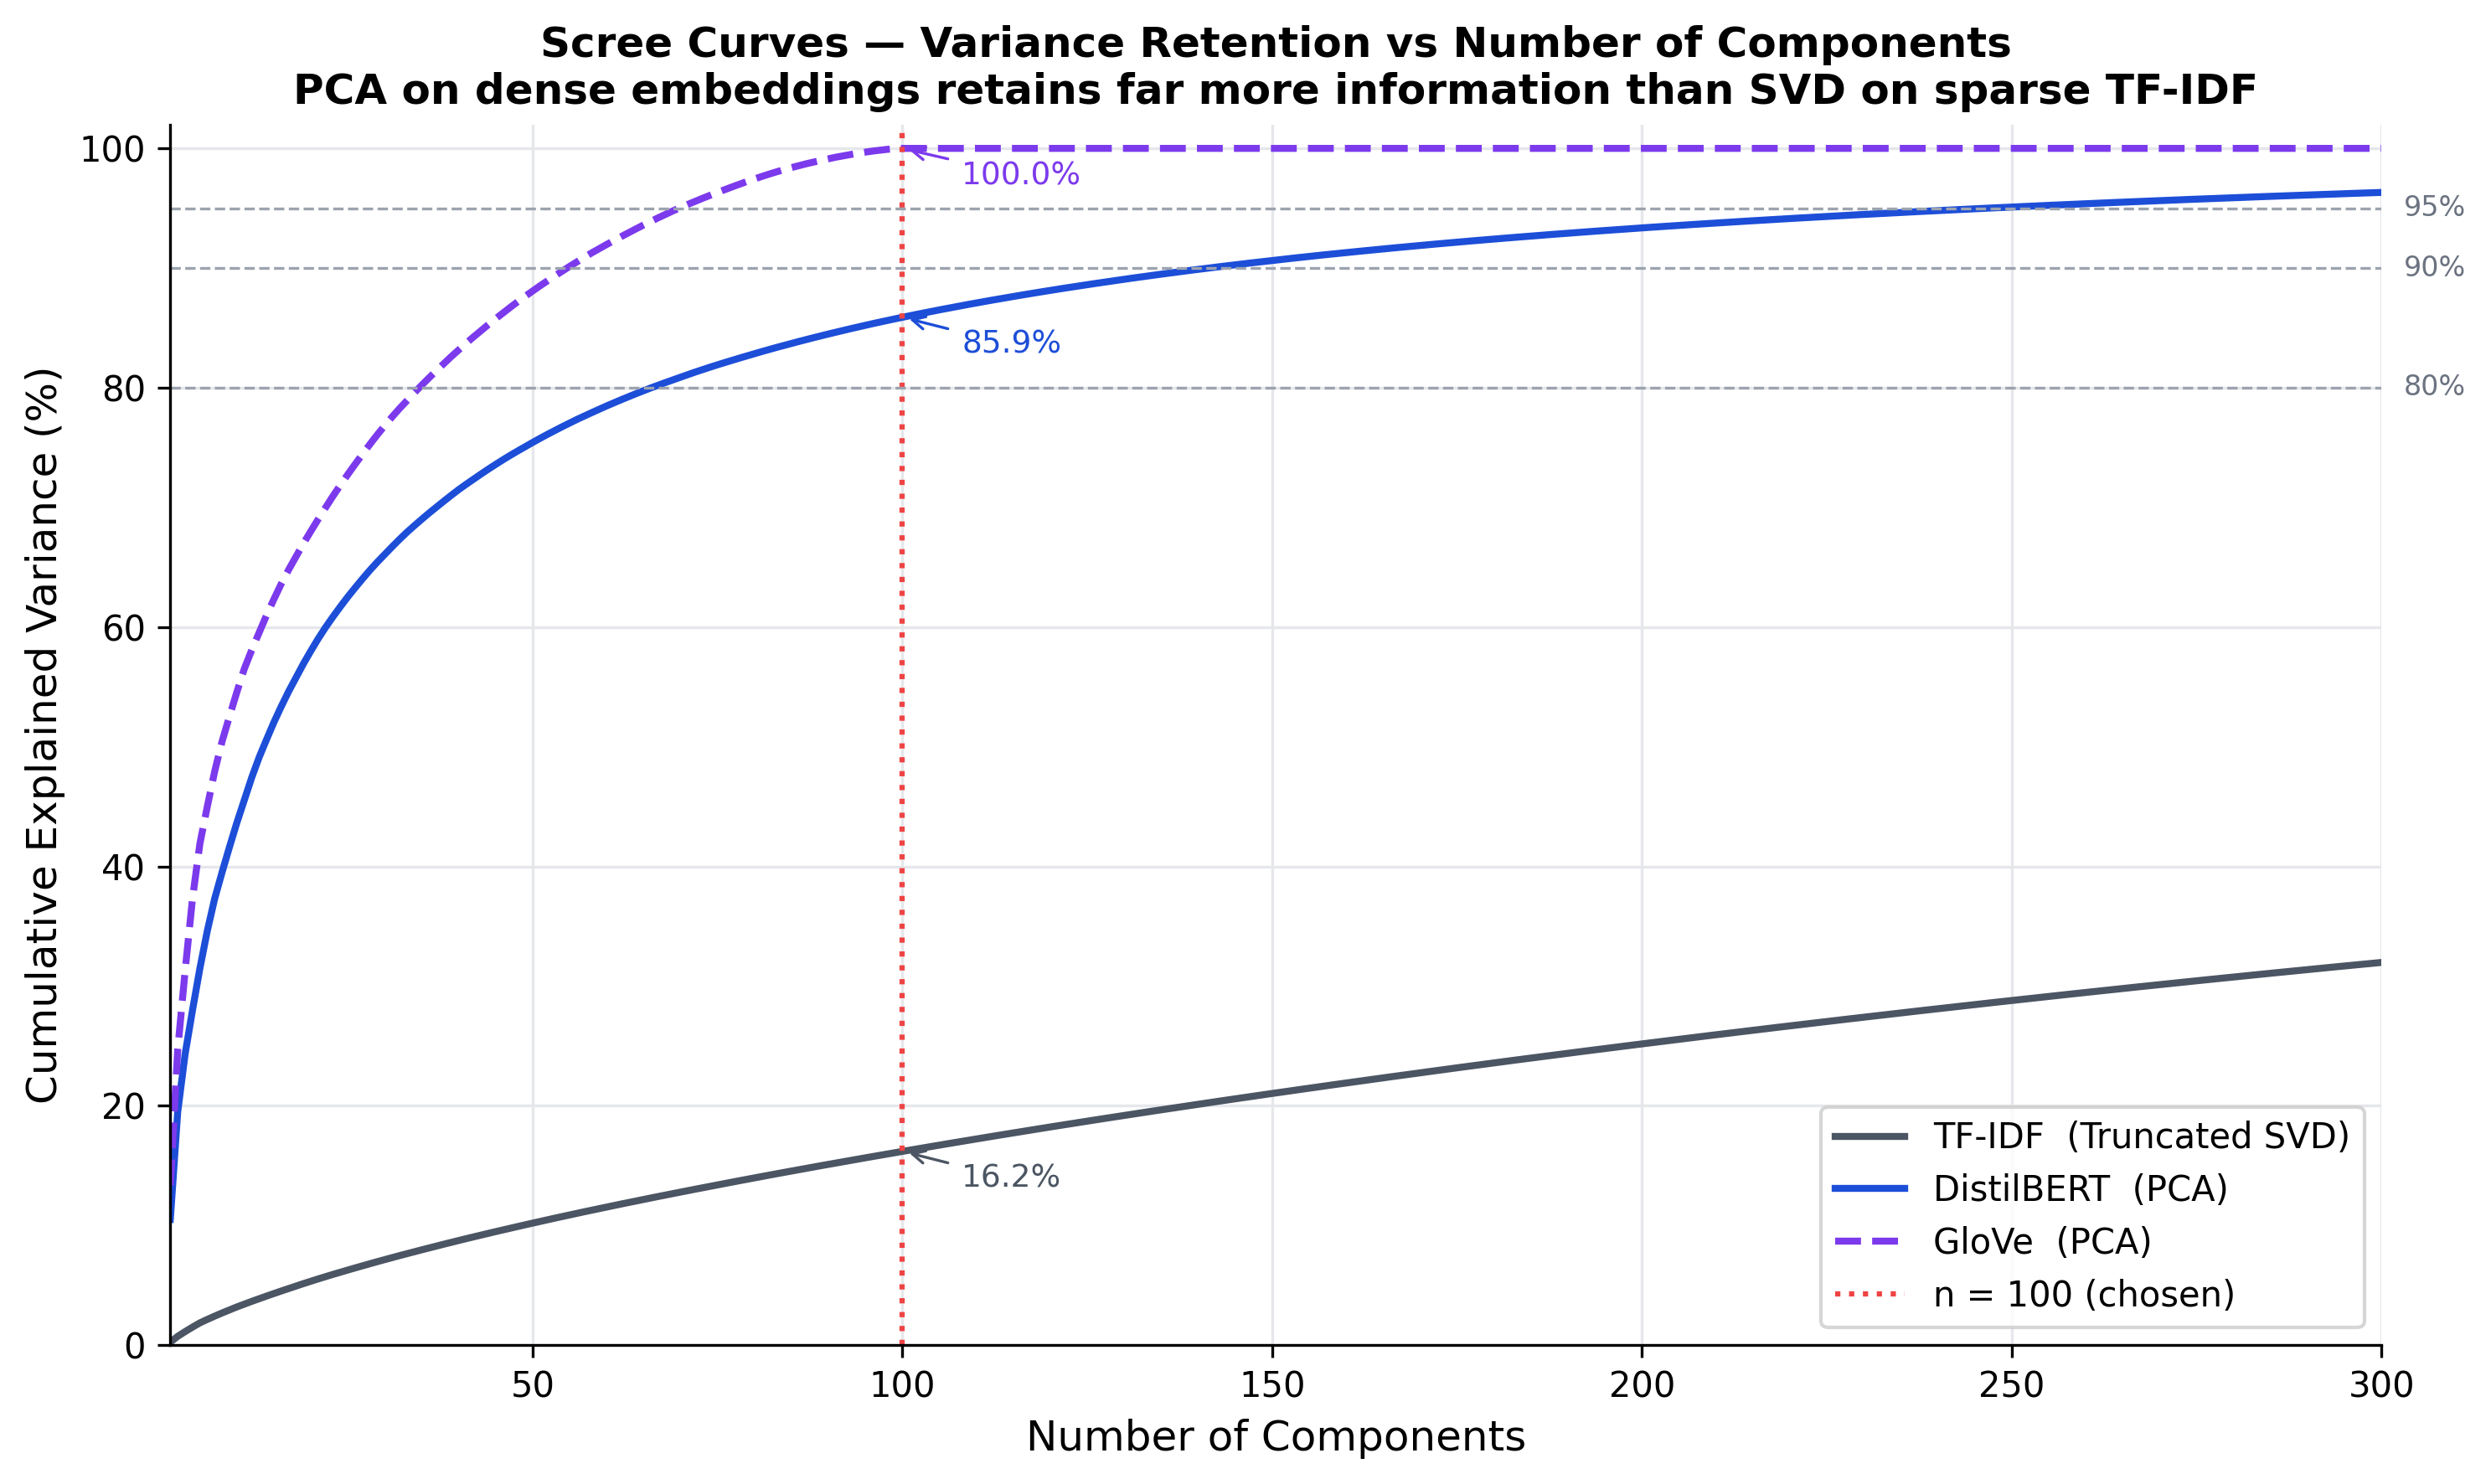
\includegraphics[width=\textwidth]{03_scree_curves.png}
    \caption{Cumulative explained variance vs number of components. Red dotted line
             marks $n=100$. PCA on DistilBERT retains \bertPcaVar{}; SVD on TF-IDF
             retains only \tfidfSvdVar{}.}
    \label{fig:scree}
\end{figure}

\subsection{Part F: Feature Space Geometry}

\begin{figure}[H]
    \centering
    \makebox[\textwidth][c]{%
        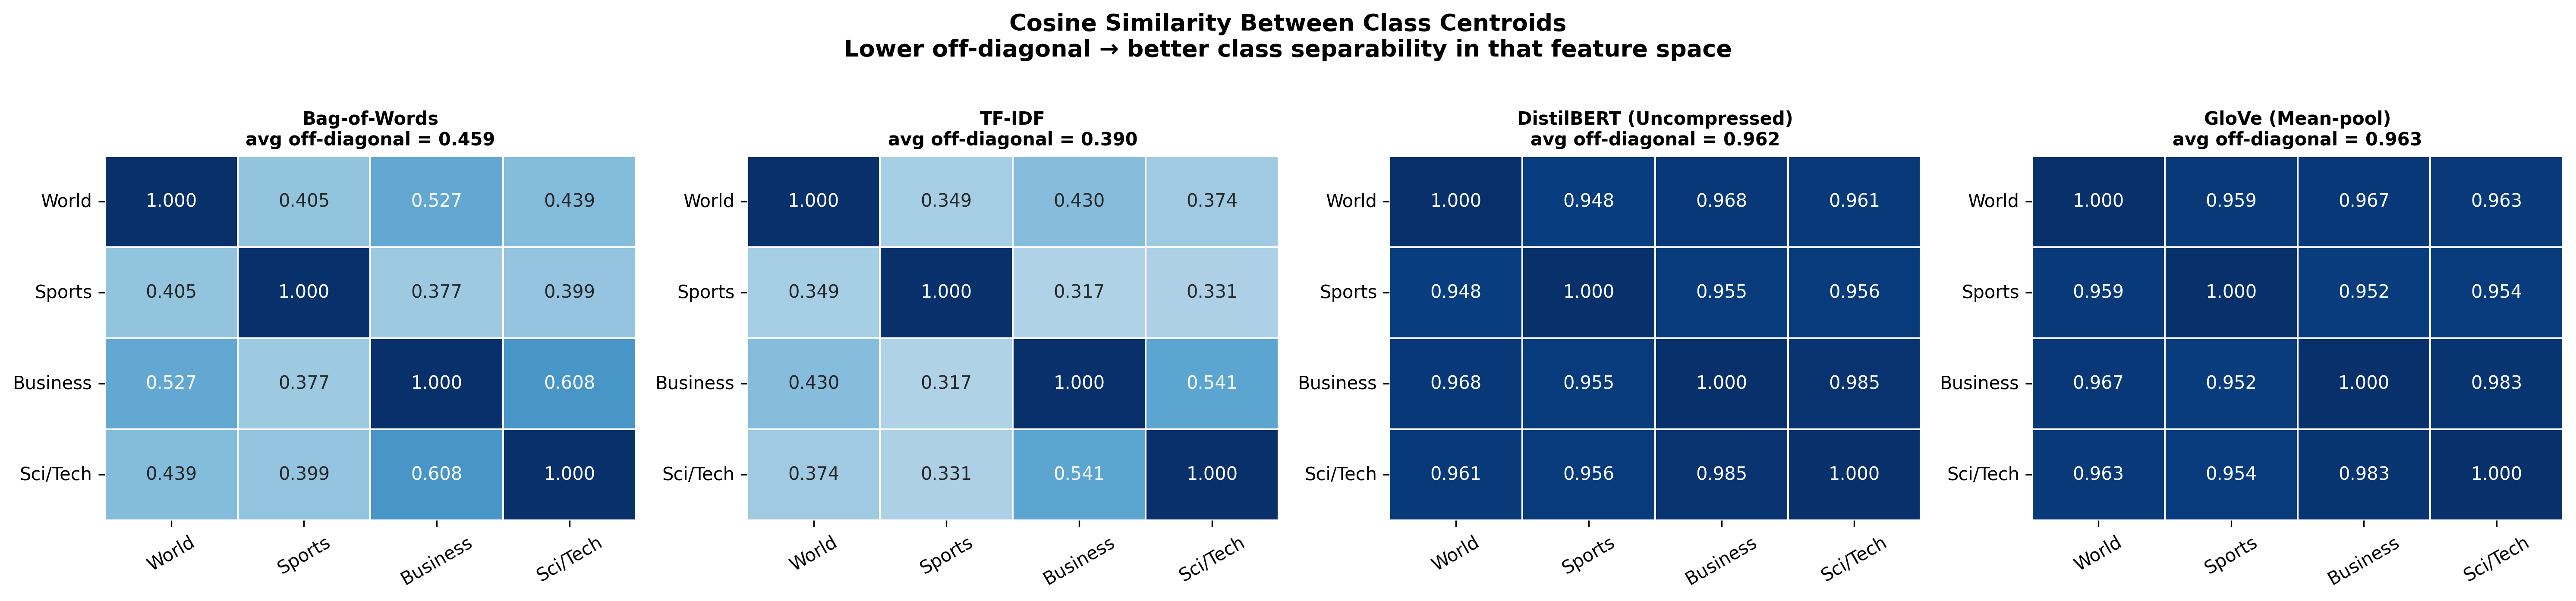
\includegraphics[width=1.15\textwidth]{06_centroid_similarity.png}%
    }
    \caption{Cosine similarity between class centroids per feature space. Lower
             off-diagonal values indicate better geometric class separation.
             DistilBERT shows the lowest average off-diagonal similarity.}
    \label{fig:centroid}
\end{figure}

\section{Experiments}

The \nSamples{} samples were partitioned into \nTrain{} training and \nTest{} test
samples (\texttt{random\_state=42}). Supervised models report \textbf{Accuracy} and
\textbf{Macro F1-score}; KMeans reports \textbf{NMI} and \textbf{ARI}.

\section{Results}

\subsection{Accuracy Comparison}

\begin{figure}[H]
    \centering
    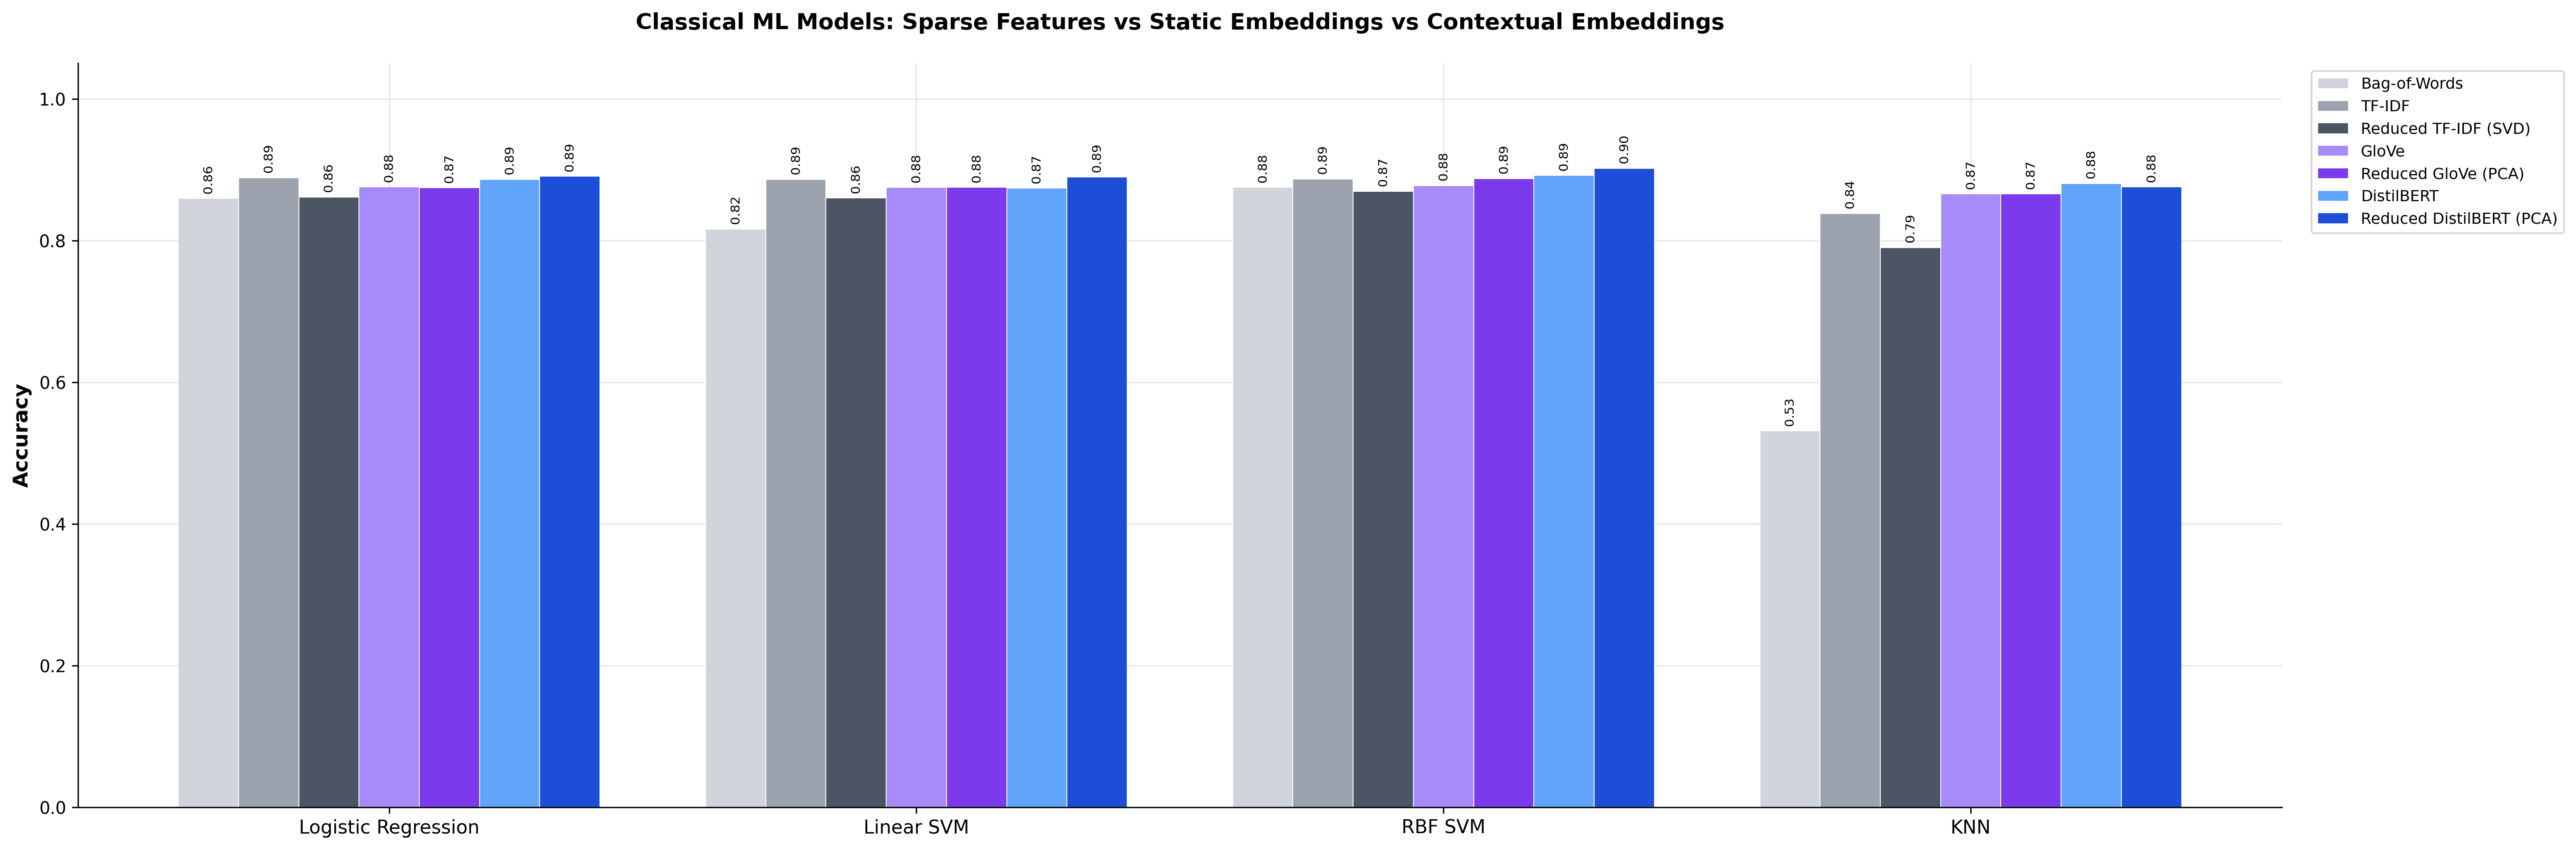
\includegraphics[width=\textwidth]{08_model_comparison.png}
    \caption{Grouped accuracy bar chart across all models and feature spaces.
             The three-tier progression Sparse $\to$ GloVe $\to$ DistilBERT
             is visible across all models.}
    \label{fig:accuracy}
\end{figure}

\subsection{Per-Class F1-Score Analysis}

\begin{figure}[H]
    \centering
    \makebox[\textwidth][c]{%
        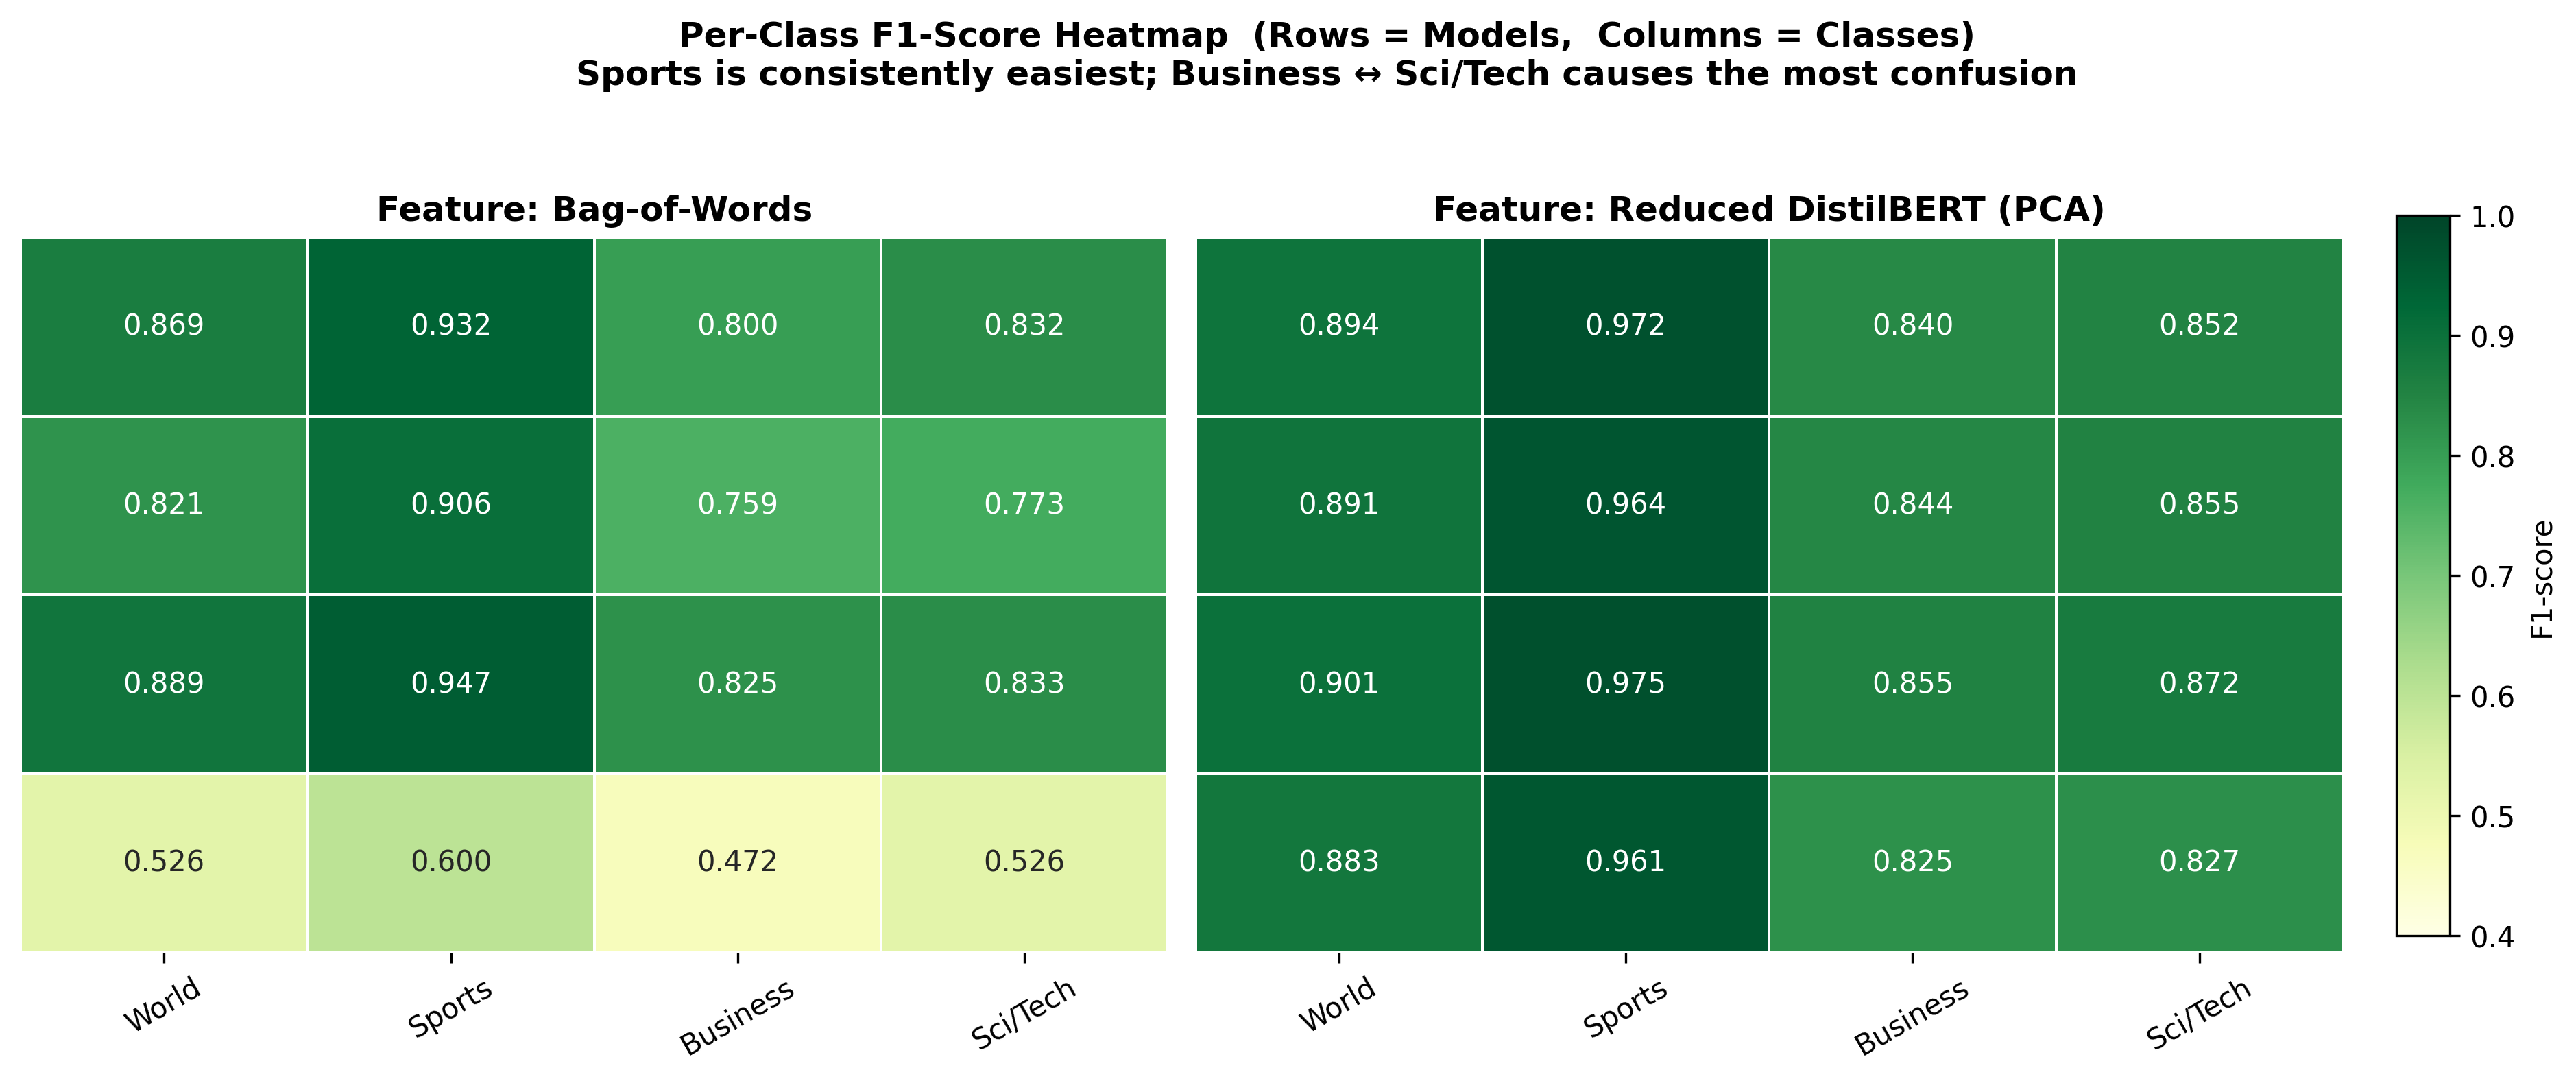
\includegraphics[width=1.1\textwidth]{09_per_class_f1_heatmap.png}%
    }
    \caption{Per-class F1 heatmap. Left: Bag-of-Words. Right: Reduced DistilBERT
             (PCA). Business--Sci/Tech confusion persists across all configurations.}
    \label{fig:heatmap}
\end{figure}

\subsection{Numerical Results}
Table~\ref{tab:results} reports all model--feature combinations.
Best accuracy per model is \textbf{bold}.

\begin{table}[H]
\centering
\caption{Accuracy and Macro F1-score for all model--feature combinations. Best accuracy per model shown in \textbf{bold}.}
\label{tab:results}
\renewcommand{\arraystretch}{1.25}
\begin{tabular}{llcc}
\toprule
\textbf{Model} & \textbf{Feature Set} & \textbf{Accuracy} & \textbf{Macro F1} \\
\midrule
Logistic Regression & Bag-of-Words (unigram) & 0.8594 & 0.8582 \\
Logistic Regression & TF-IDF (unigram+bigram) & 0.8888 & 0.8874 \\
Logistic Regression & Reduced TF-IDF (SVD, 100d) & 0.8612 & 0.8596 \\
Logistic Regression & GloVe mean-pool (100d) & 0.8756 & 0.8745 \\
Logistic Regression & Reduced GloVe (PCA, 100d) & 0.8744 & 0.8733 \\
Logistic Regression & DistilBERT (768d) & 0.8862 & 0.8854 \\
Logistic Regression & Reduced DistilBERT (PCA, 100d) & \textbf{0.8906} & 0.8895 \\
\midrule
Linear SVM & Bag-of-Words (unigram) & 0.8163 & 0.8145 \\
Linear SVM & TF-IDF (unigram+bigram) & 0.8862 & 0.8851 \\
Linear SVM & Reduced TF-IDF (SVD, 100d) & 0.8600 & 0.8585 \\
Linear SVM & GloVe mean-pool (100d) & 0.8750 & 0.8739 \\
Linear SVM & Reduced GloVe (PCA, 100d) & 0.8750 & 0.8739 \\
Linear SVM & DistilBERT (768d) & 0.8738 & 0.8723 \\
Linear SVM & Reduced DistilBERT (PCA, 100d) & \textbf{0.8894} & 0.8884 \\
\midrule
RBF SVM & Bag-of-Words (unigram) & 0.8750 & 0.8737 \\
RBF SVM & TF-IDF (unigram+bigram) & 0.8869 & 0.8856 \\
RBF SVM & Reduced TF-IDF (SVD, 100d) & 0.8694 & 0.8682 \\
RBF SVM & GloVe mean-pool (100d) & 0.8775 & 0.8766 \\
RBF SVM & Reduced GloVe (PCA, 100d) & 0.8875 & 0.8866 \\
RBF SVM & DistilBERT (768d) & 0.8919 & 0.8908 \\
RBF SVM & Reduced DistilBERT (PCA, 100d) & \textbf{0.9019} & 0.9009 \\
\midrule
KNN & Bag-of-Words (unigram) & 0.5312 & 0.5309 \\
KNN & TF-IDF (unigram+bigram) & 0.8381 & 0.8361 \\
KNN & Reduced TF-IDF (SVD, 100d) & 0.7900 & 0.7876 \\
KNN & GloVe mean-pool (100d) & 0.8656 & 0.8640 \\
KNN & Reduced GloVe (PCA, 100d) & 0.8656 & 0.8640 \\
KNN & DistilBERT (768d) & \textbf{0.8806} & 0.8792 \\
KNN & Reduced DistilBERT (PCA, 100d) & 0.8756 & 0.8741 \\
\bottomrule
\end{tabular}
\end{table}

\subsection{Feature Space Geometry}

\begin{figure}[H]
    \centering
    \makebox[\textwidth][c]{%
        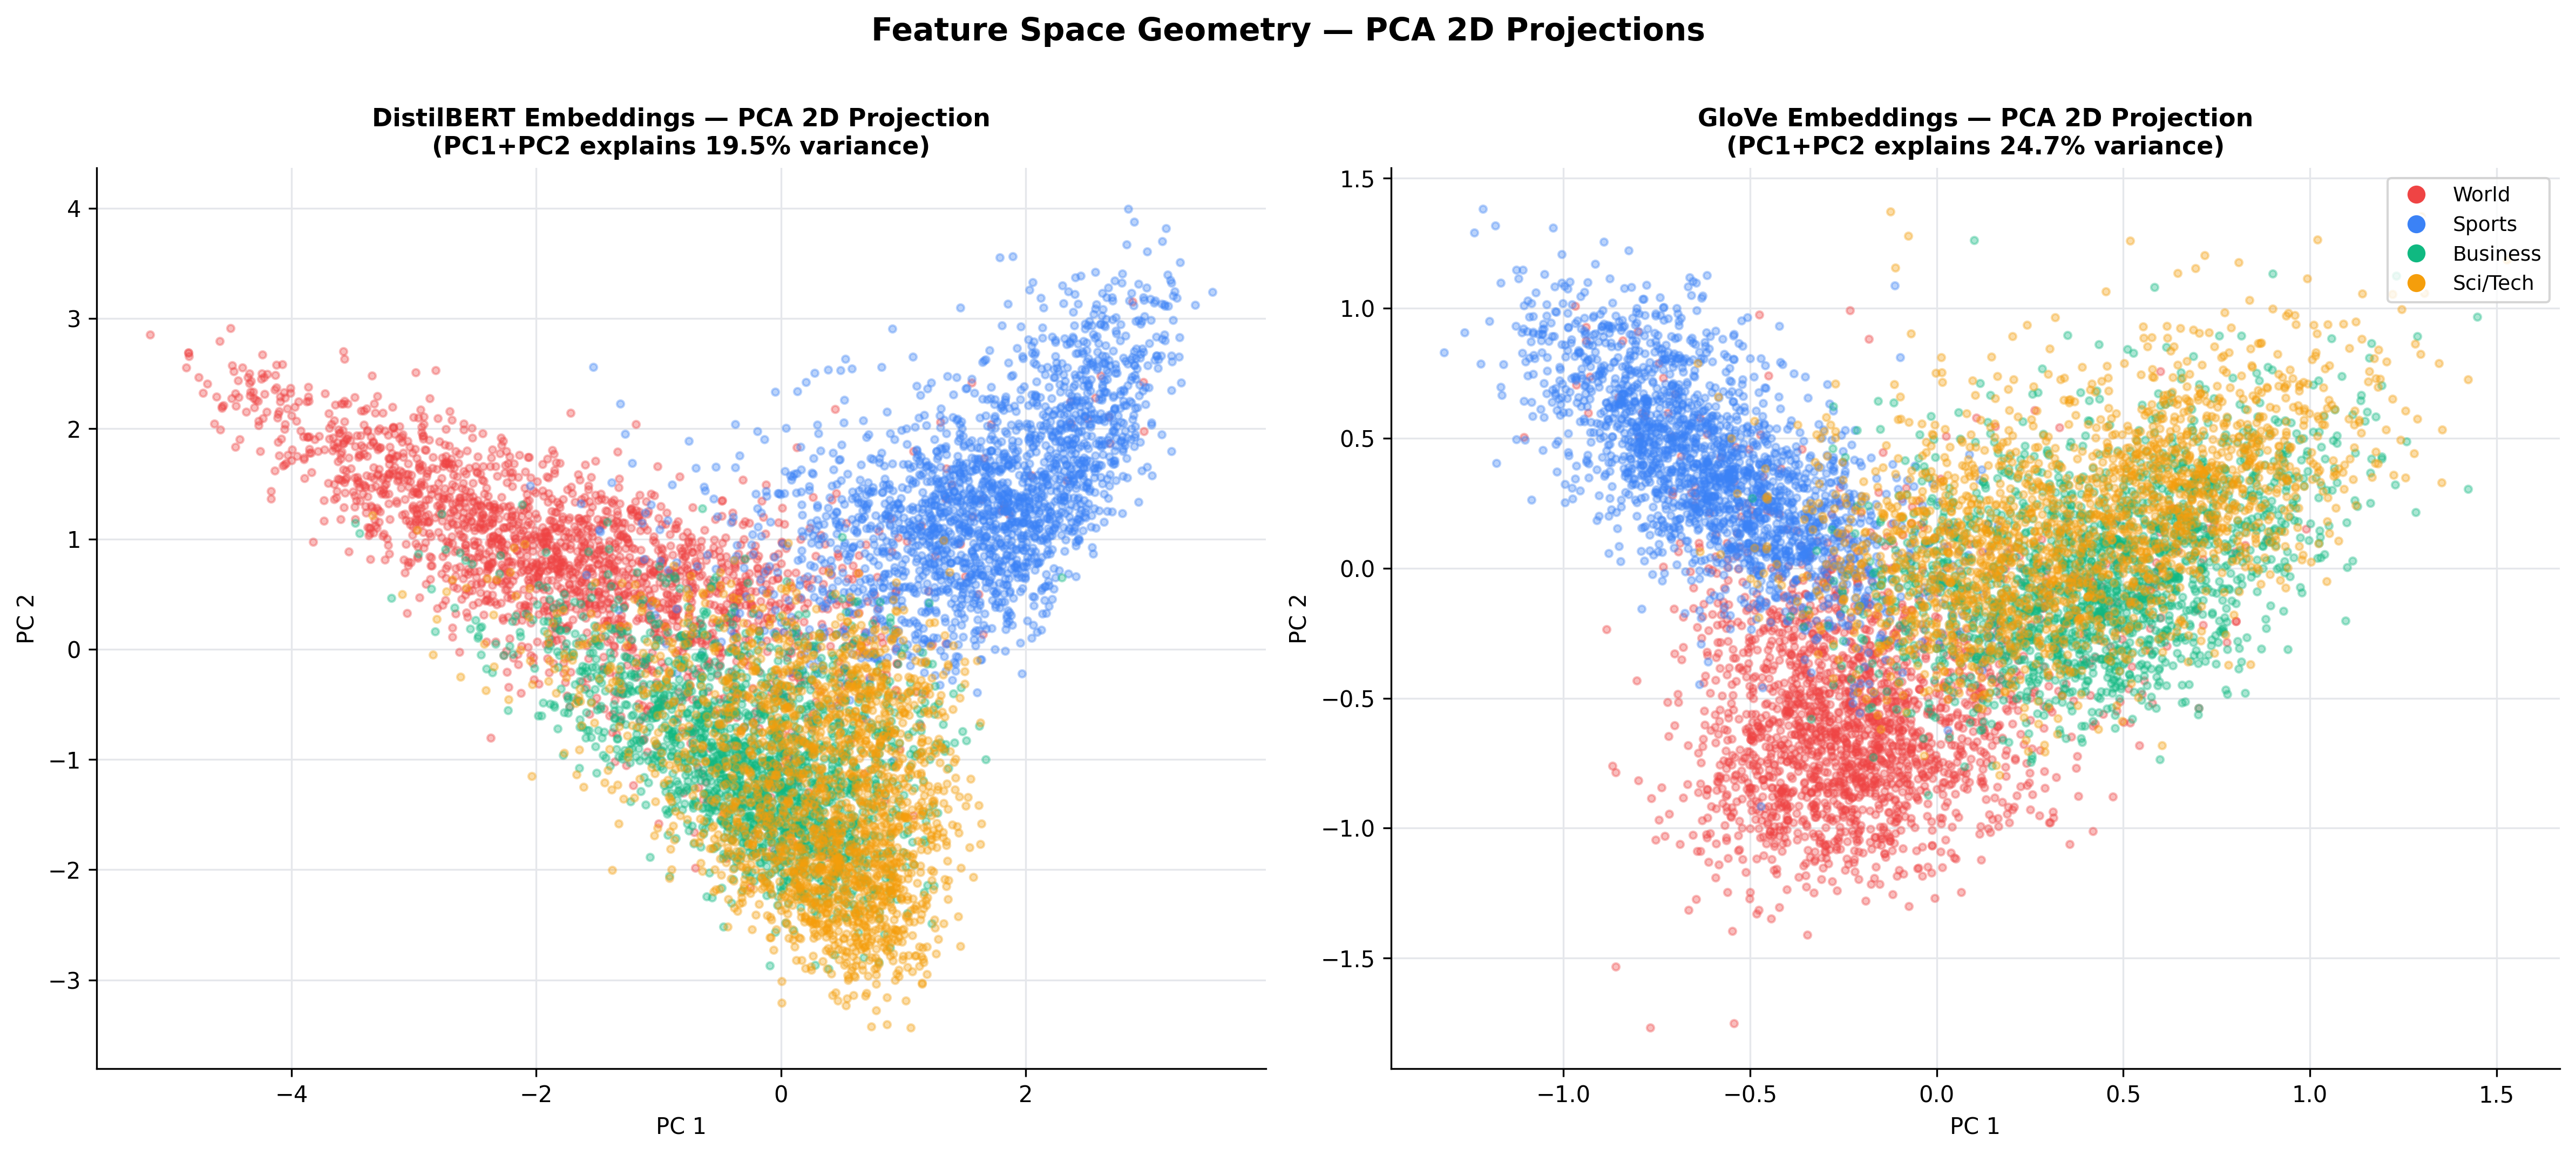
\includegraphics[width=1.15\textwidth]{04_pca_scatter.png}%
    }
    \caption{PCA 2D projections. Left: DistilBERT. Right: GloVe (partial separation,
             less structured than DistilBERT but more than BoW).}
    \label{fig:pca}
\end{figure}

\begin{figure}[H]
    \centering
    \makebox[\textwidth][c]{%
        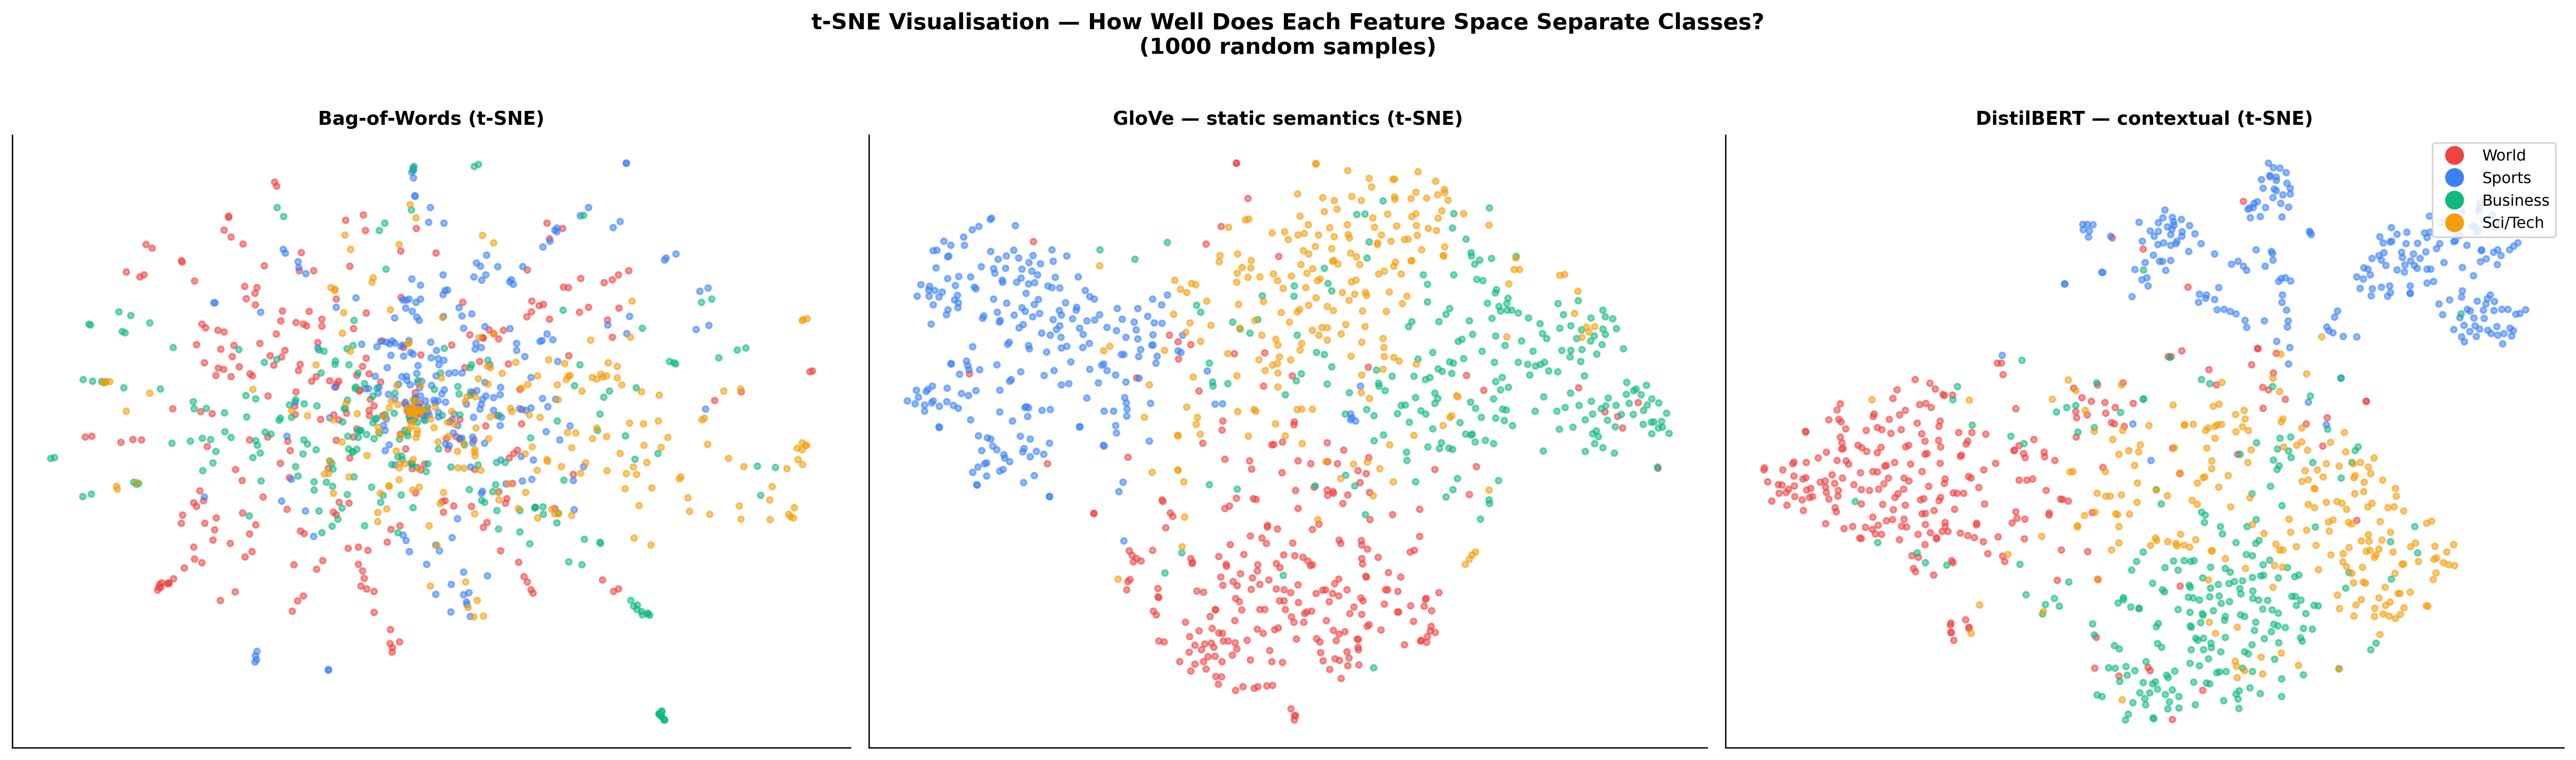
\includegraphics[width=1.15\textwidth]{05_tsne_comparison.png}%
    }
    \caption{t-SNE (1,000 samples). BoW (left): indistinguishable blob.
             GloVe (centre): partial cluster emergence. DistilBERT (right):
             tight well-separated clusters before any classifier is applied.}
    \label{fig:tsne}
\end{figure}

\subsection{Confusion Matrix}

\begin{figure}[H]
    \centering
    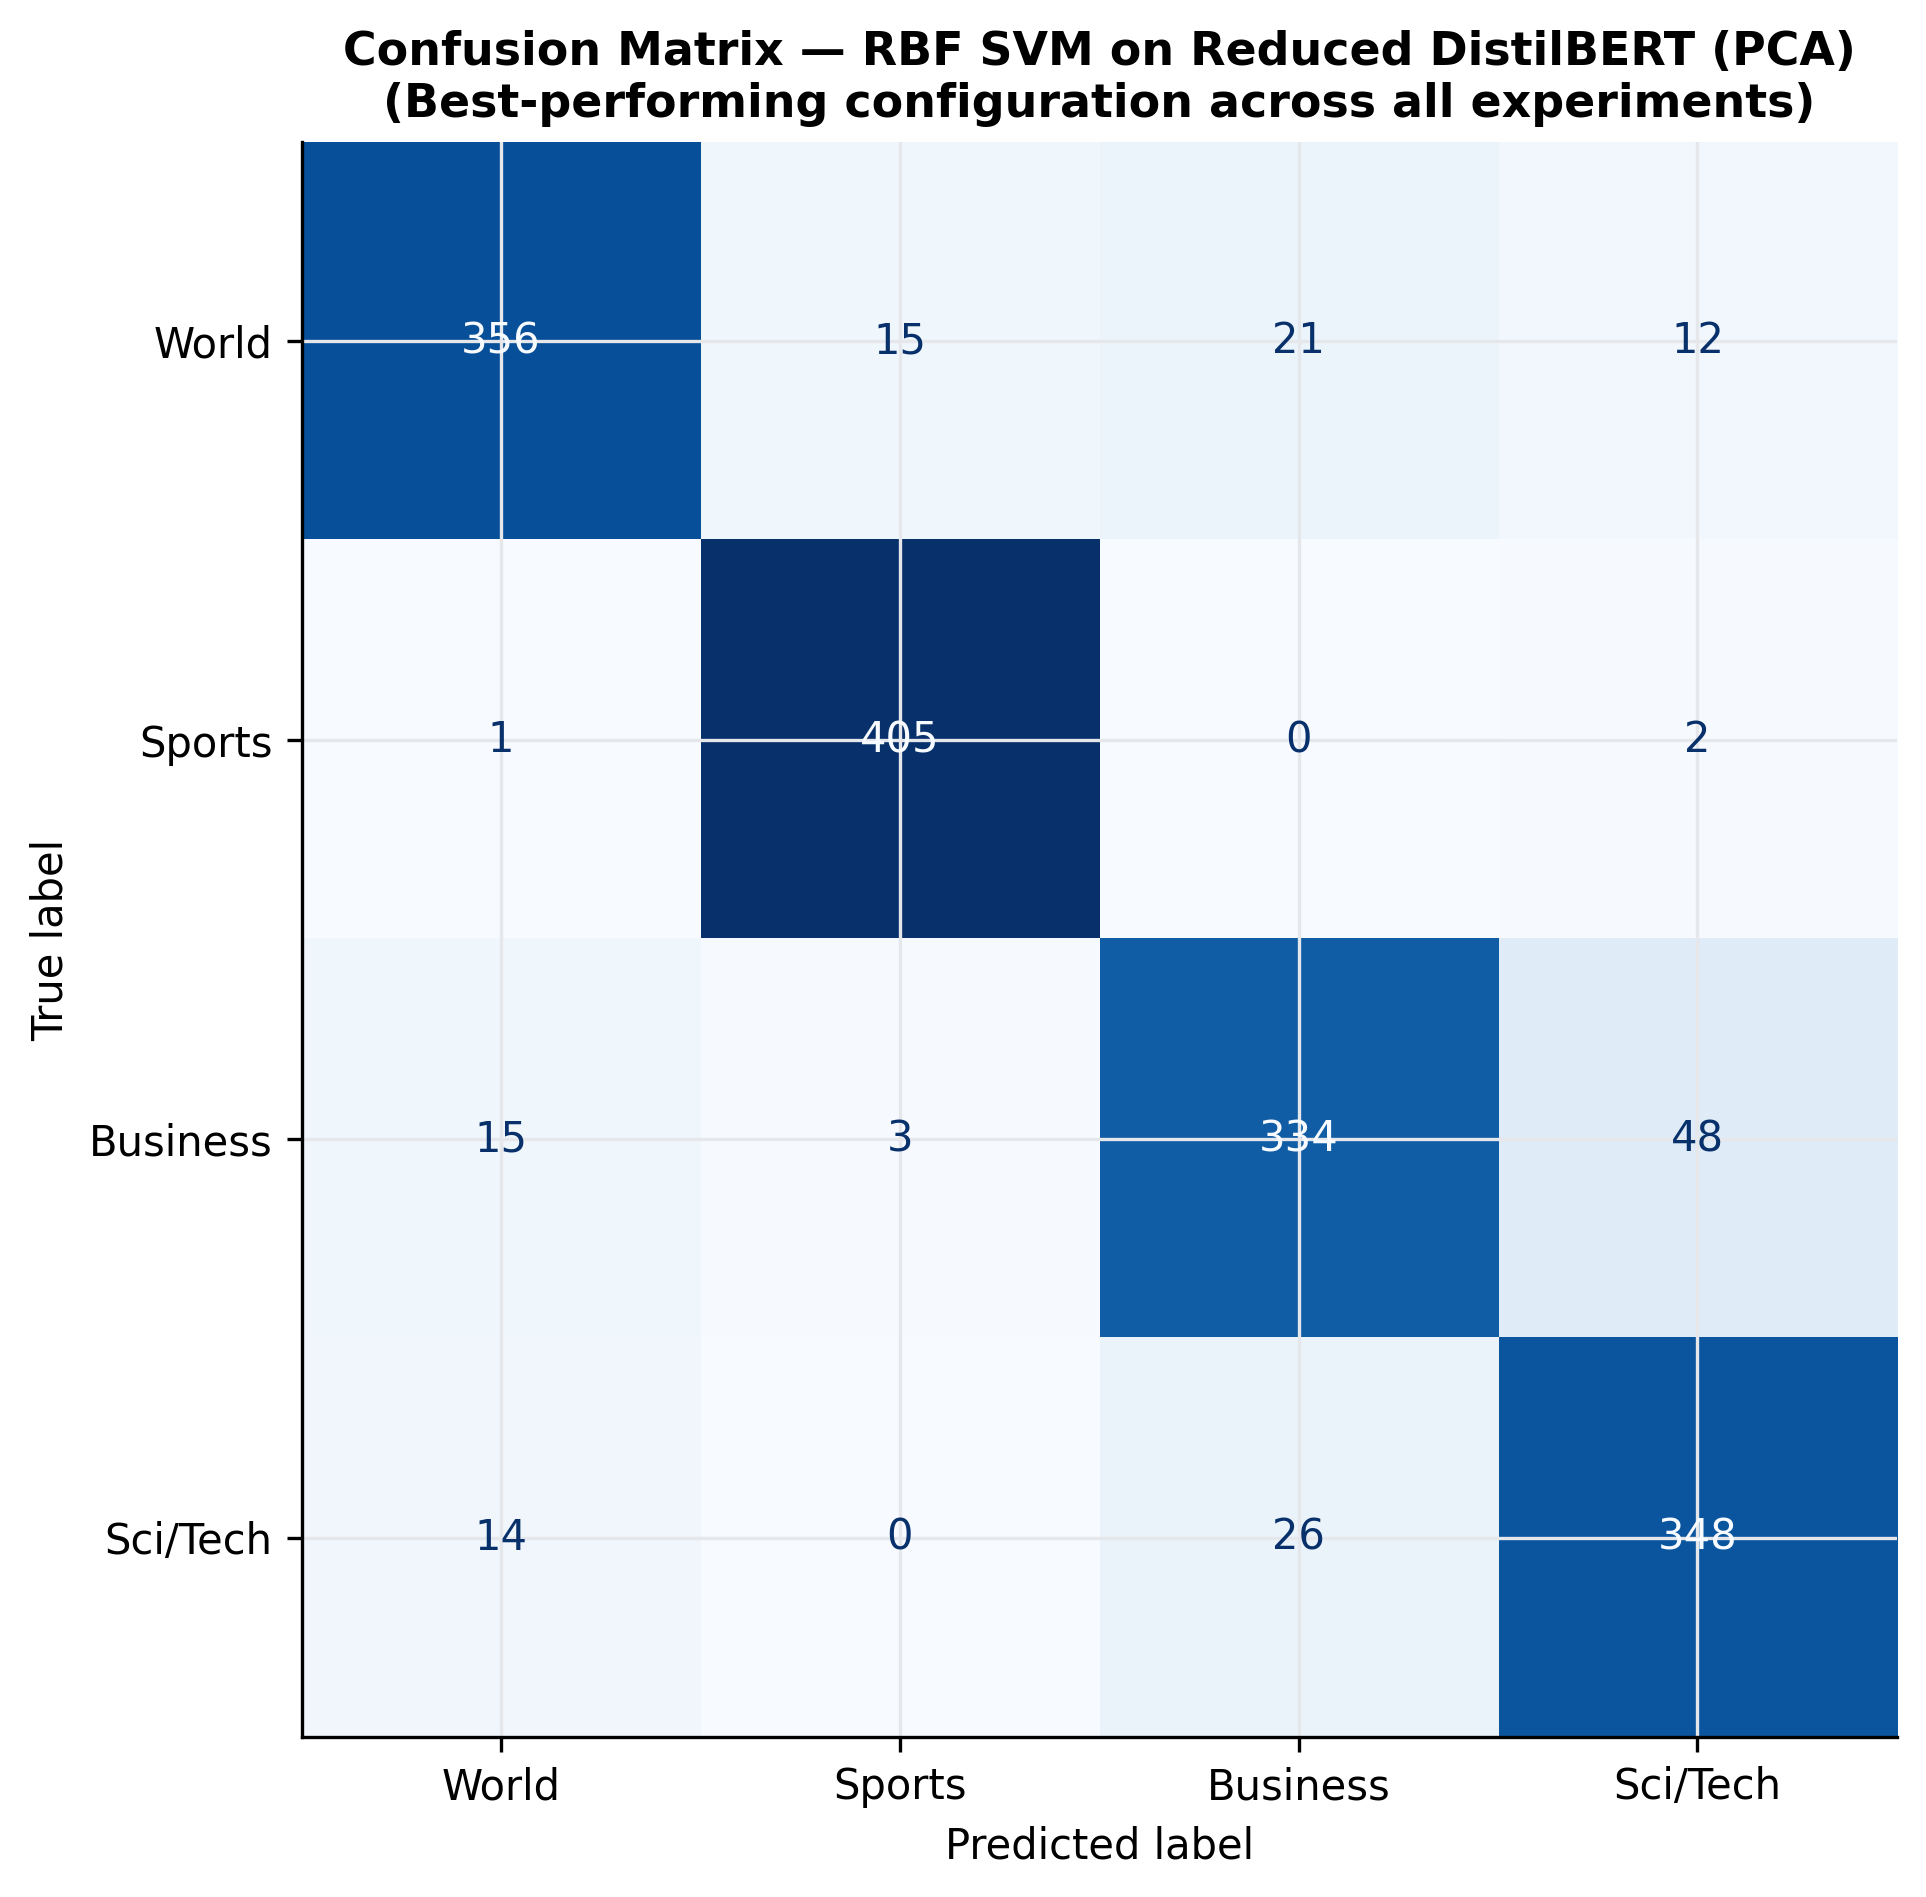
\includegraphics[width=0.80\textwidth]{07_confusion_matrix.png}
    \caption{Confusion matrix for \bestModel{} on \bestFeat{}
             (\bestAcc{} accuracy which is best overall).
             Sports: \cmSportsCorrect/\cmSportsTotal{} correct.
             Primary error: \cmBizToSci{} Business articles misclassified as Sci/Tech.}
    \label{fig:cm}
\end{figure}

\subsection{KMeans Unsupervised Quality}

\begin{figure}[H]
    \centering
    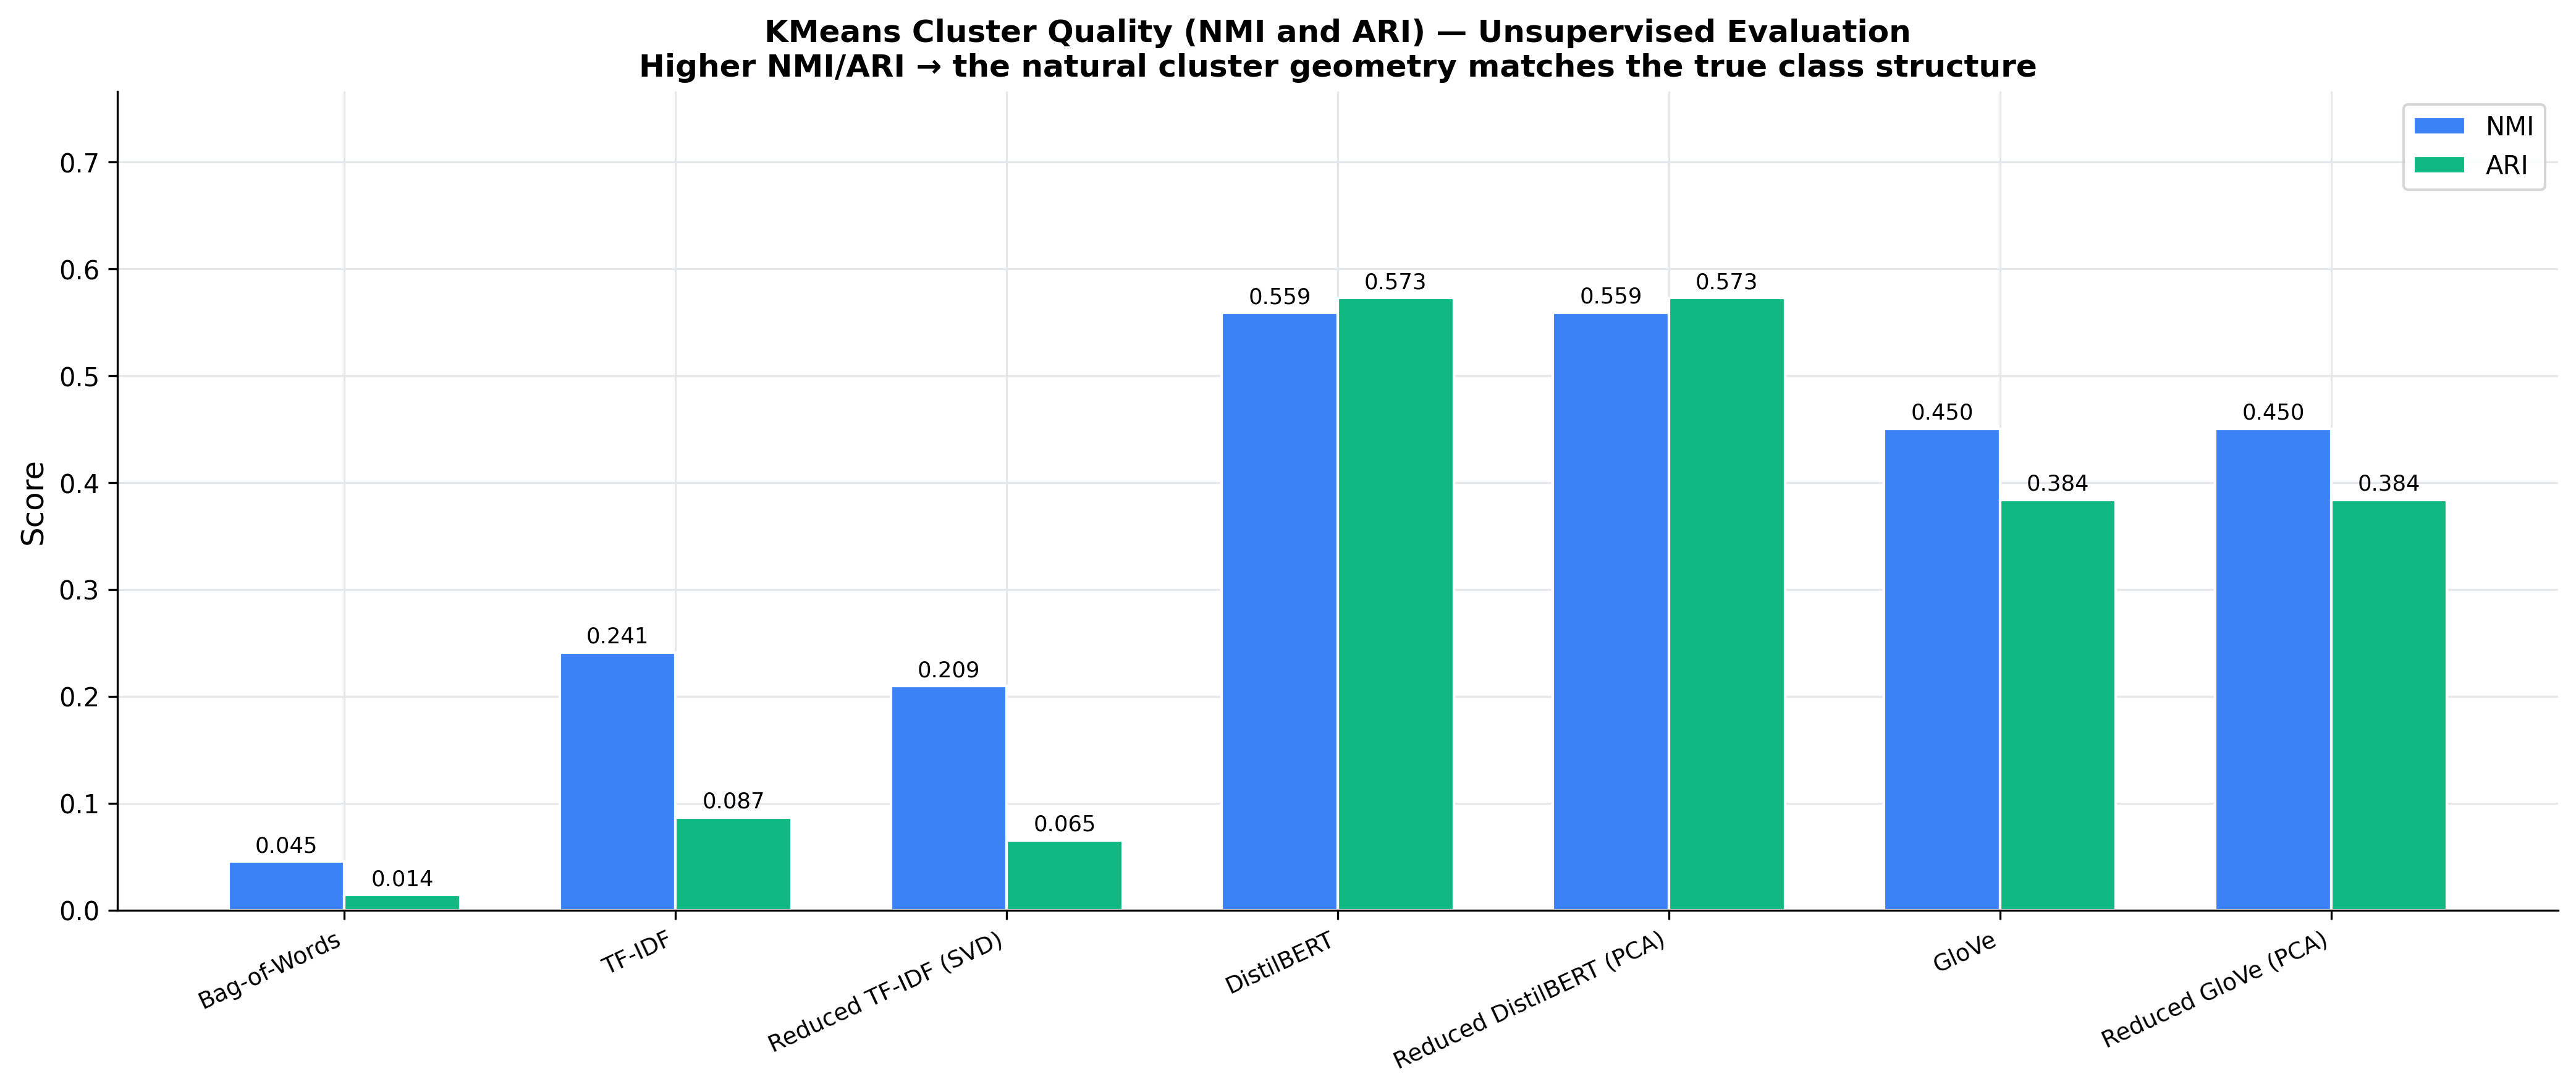
\includegraphics[width=\textwidth]{11_kmeans_quality.png}
    \caption{KMeans NMI and ARI across all feature spaces.
             DistilBERT: NMI $=$ \kmBertNmi, ARI $=$ \kmBertAri.
             BoW: NMI $=$ \kmBowNmi, ARI $=$ \kmBowAri.}
    \label{fig:kmeans}
\end{figure}

\section{Discussion}

\subsection{Curse of Dimensionality}
Most clearly illustrated by KNN: on \vocabSize{} sparse BoW dimensions, accuracy
collapses to \knnBoWAcc{}. With dense 768-dimensional DistilBERT vectors, the same
KNN achieves \knnBertAcc{} which is a \knnJumpPP{}-point jump from a feature change alone.

\subsection{Dimensionality Reduction Efficacy}
PCA retains \bertPcaVar{} of DistilBERT variance in 100 components, allowing
Logistic Regression to improve (\lrBertImprove{}). SVD on TF-IDF retains only
\tfidfSvdVar{}, causing a moderate drop (\lrTfidfDrop{}). Compression is safe for
dense structured embeddings, destructive for sparse representations.

\subsection{Feature Geometry}
The t-SNE comparison (Figure~\ref{fig:tsne}) and centroid heatmaps
(Figure~\ref{fig:centroid}) together explain the accuracy gap geometrically.
BoW centroids show substantially higher off-diagonal cosine similarity than
DistilBERT centroids; the gap is a property of the feature space, not the classifier.

\subsection{Class-level Confusion}
Sports is easiest due to domain-specific vocabulary. \cmBizToSci{} Business articles
are misclassified as Sci/Tech because modern tech-company news straddles both domains.
This difficulty hierarchy is \textit{preserved} across all feature spaces.

\subsection{KMeans as Unsupervised Baseline}
DistilBERT achieves NMI $=$ \kmBertNmi{} and ARI $=$ \kmBertAri{} without any
classifier, versus NMI $=$ \kmBowNmi{} and ARI $=$ \kmBowAri{} for BoW. The
separation in Figures~\ref{fig:pca} and~\ref{fig:tsne} is genuine and measurable.

\subsection{GloVe as Semantic Bridge}
Despite dense vectors and word-level semantics, RBF SVM achieves only \gloveRbfAcc{}
on GloVe versus \rbfBertPcaAcc{} on Reduced DistilBERT. The gap isolates the
precise contribution of \textit{contextual disambiguation}, not density.

The hierarchy BoW $<$ TF-IDF $<$ GloVe $<$ DistilBERT maps directly to:
no semantics $\to$ bigram co-occurrence $\to$ static word semantics $\to$
contextual sentence semantics.

\subsection{Data Efficiency (Learning Curves)}

\begin{figure}[H]
    \centering
    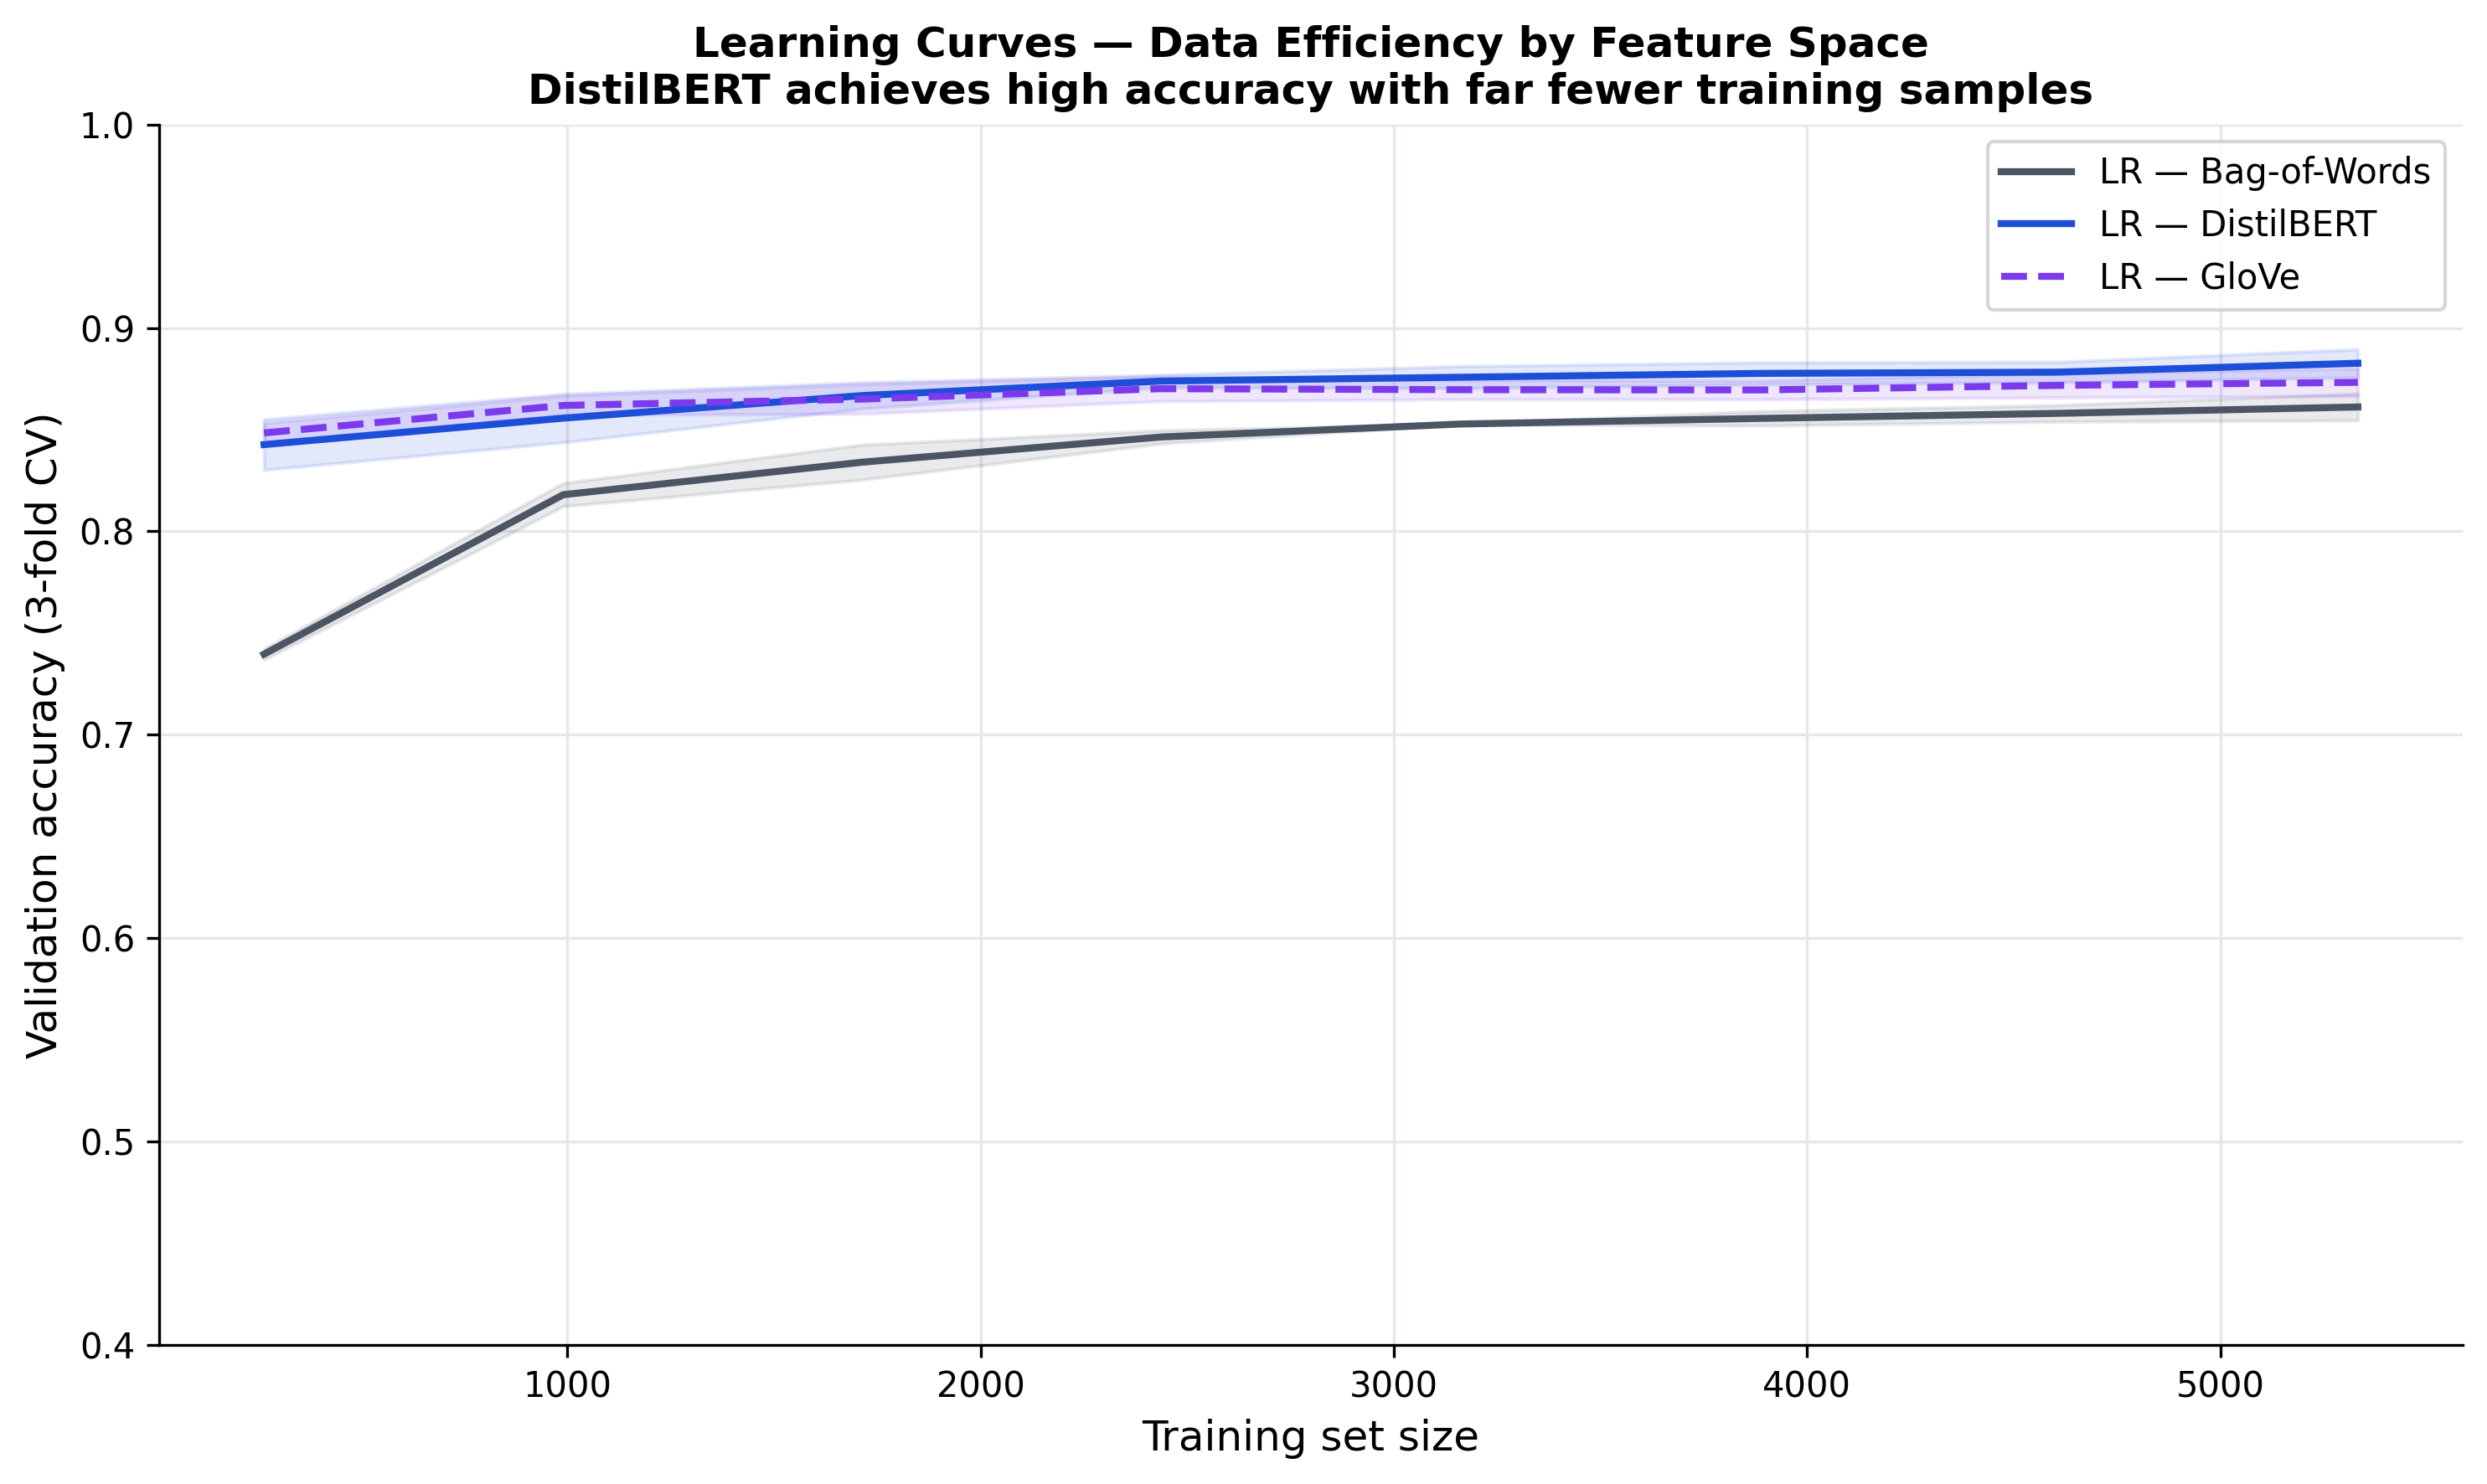
\includegraphics[width=\textwidth]{10_learning_curves.png}
    \caption{Cross-validated (3-fold) learning curves for Logistic Regression.
             DistilBERT achieves high accuracy with far fewer training samples.
             BoW continues improving throughout; DistilBERT saturates early.}
    \label{fig:lc}
\end{figure}

DistilBERT achieves high accuracy with significantly fewer training samples than BoW,
demonstrating structural knowledge that reduces labelled data requirements.

\subsection{Accuracy--Efficiency Trade-off}

\begin{figure}[H]
    \centering
    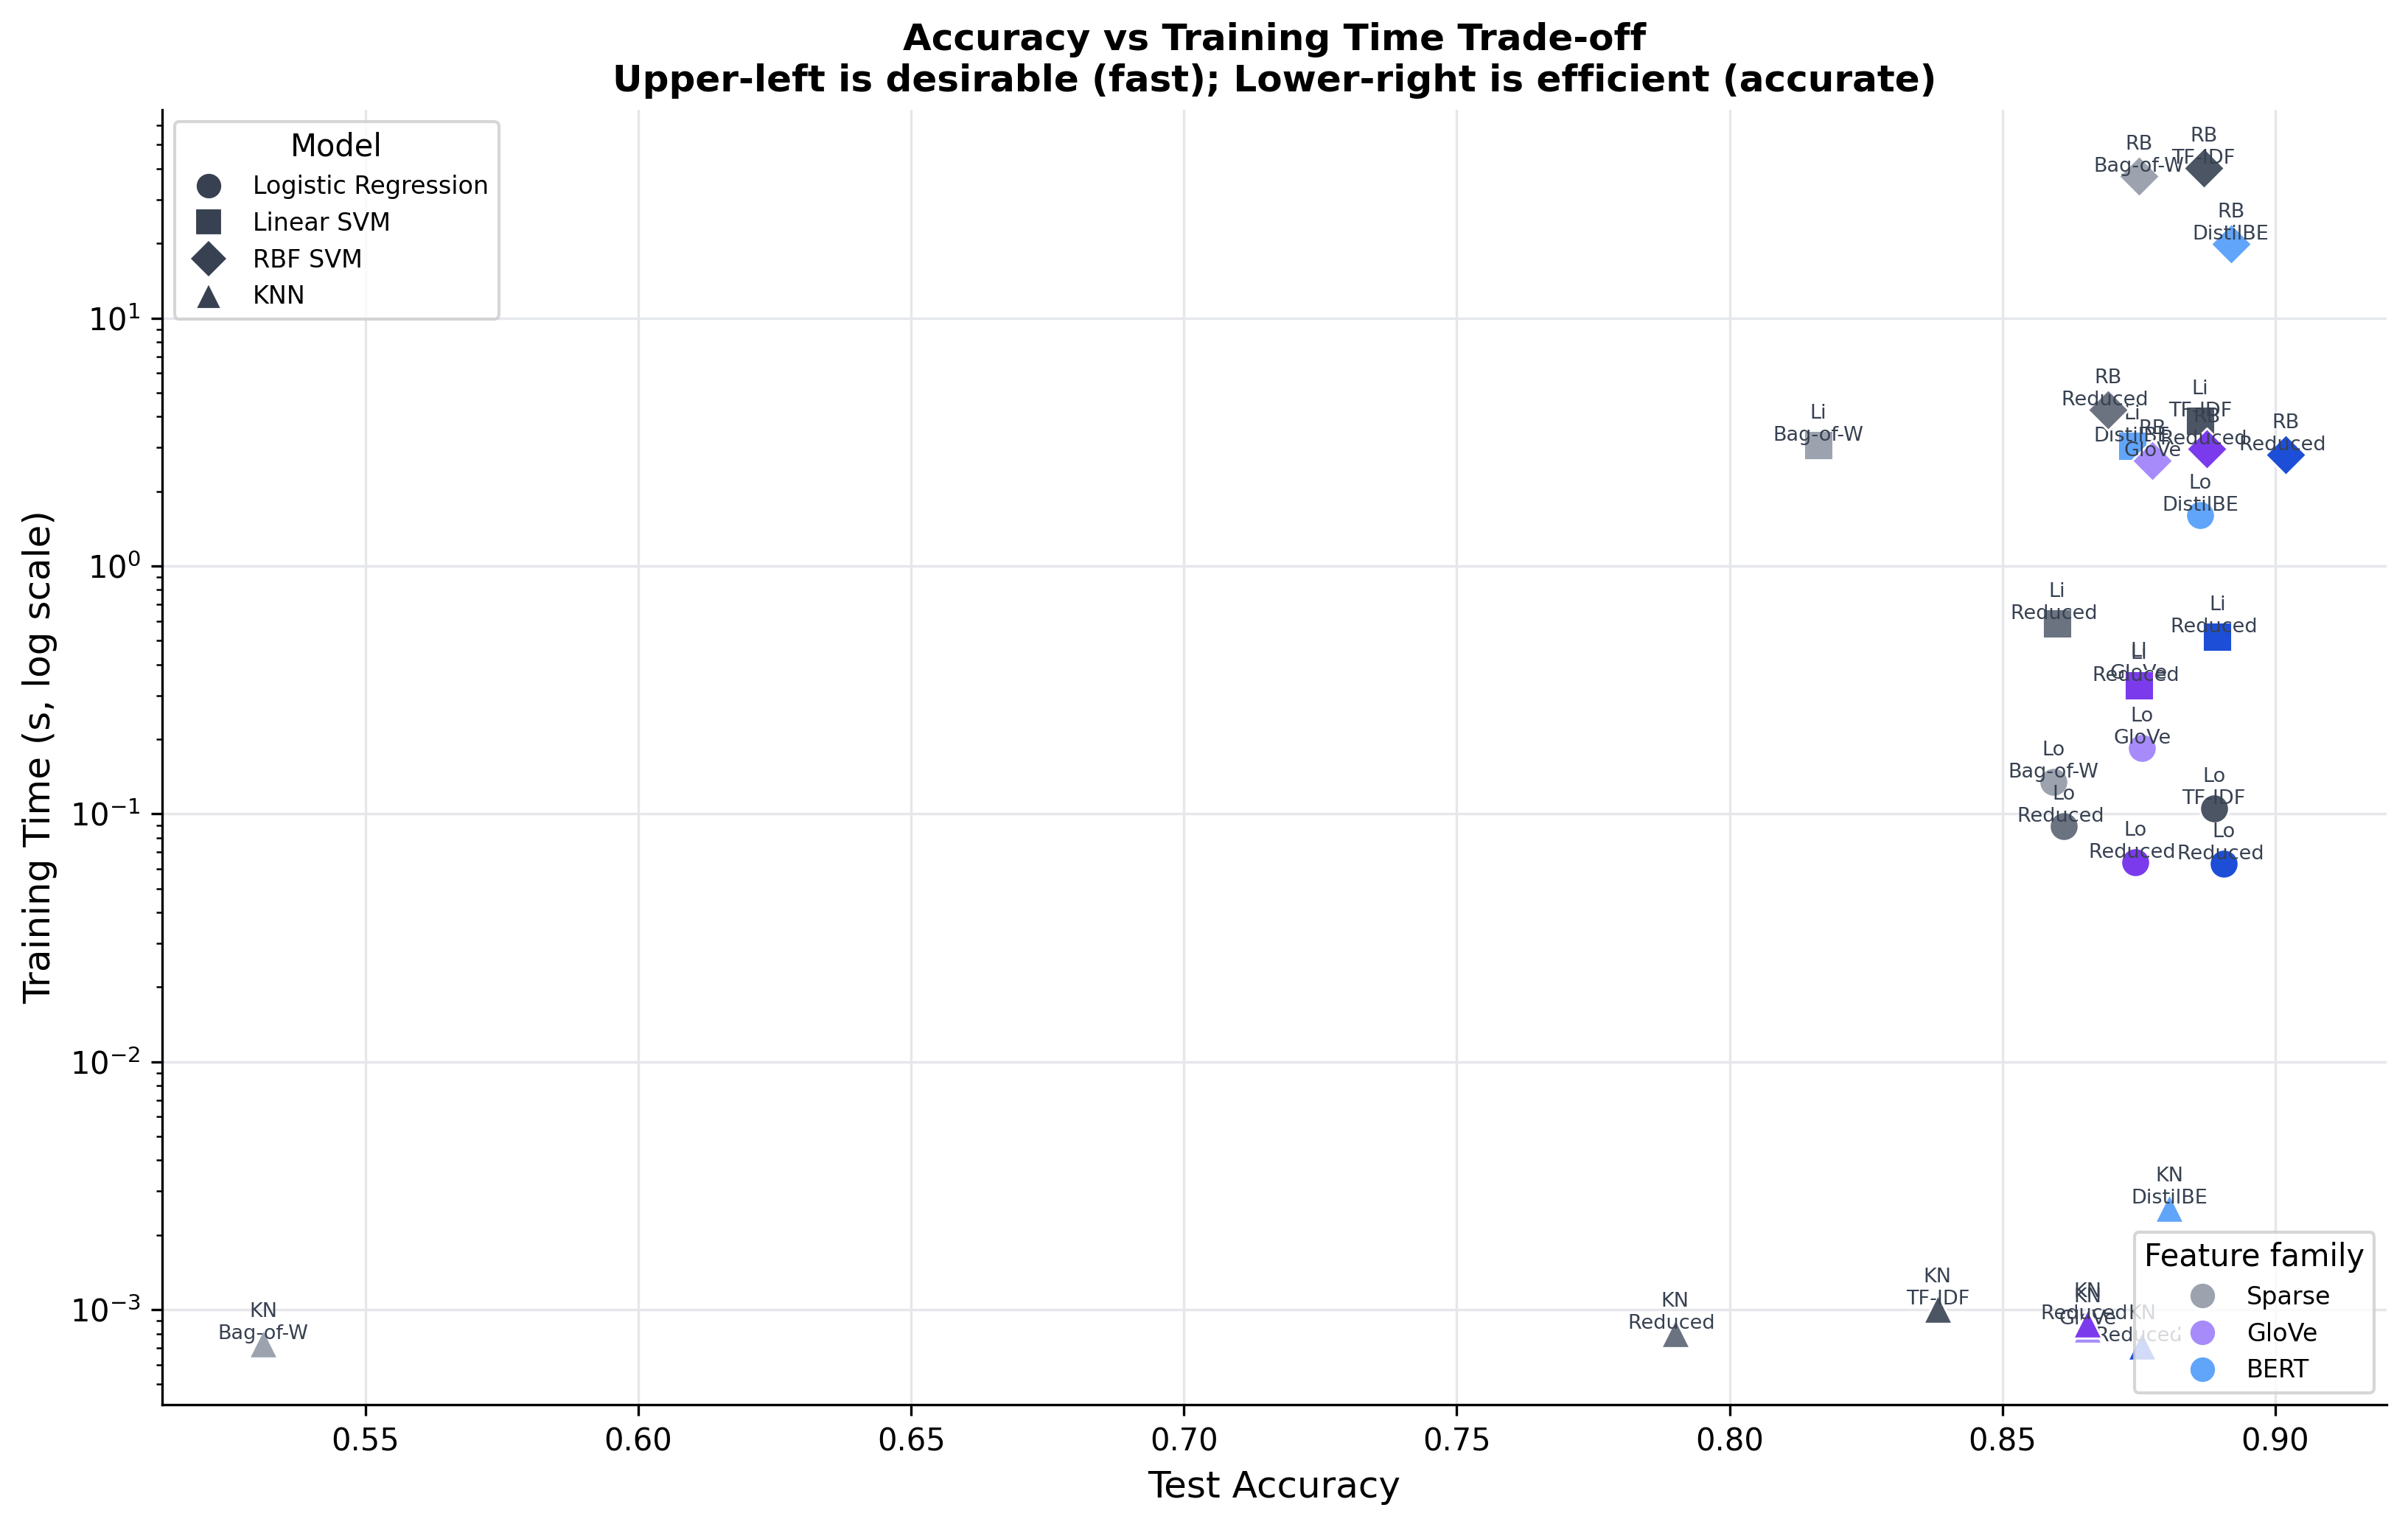
\includegraphics[width=\textwidth]{12_time_accuracy_scatter.png}
    \caption{Accuracy vs training time (log scale). Logistic Regression on Reduced
             DistilBERT (\lrBertPcaAcc{}) sits on the efficiency frontier.}
    \label{fig:scatter}
\end{figure}

Logistic Regression on Reduced DistilBERT (PCA) at \lrBertPcaAcc{} offers near-top
accuracy at low training cost. \bestModel{} achieves the overall best at \bestAcc{}.

\subsection{Limitations}
\begin{enumerate}
    \item \textbf{Single train-test split.} One 80/20 split (\texttt{random\_state=42});
          cross-validation only in learning curves.
    \item \textbf{No hyperparameter search.} Default sklearn parameters throughout.
    \item \textbf{GloVe mean-pooling.} Arithmetic mean ignores word order.
    \item \textbf{DistilBERT CLS token.} Mean-pooling across all token positions
          is often more robust; not explored here.
\end{enumerate}

\section{Conclusion and Learnings}

This project demonstrated that classical ML performance is fundamentally bounded by
input feature quality. The three-tier comparison of sparse features, GloVe, DistilBERT;
establishes a hierarchy corresponding directly to representational richness.

The best-performing configuration is \bestModel{} on \bestFeat{} at \bestAcc{}
(Macro F1 $=$ \bestFscore{}). PCA on DistilBERT retains \bertPcaVar{} in 100
components while SVD on TF-IDF retains only \tfidfSvdVar{}, making compression
viable for embeddings but destructive for sparse features. The learning curves confirm
that DistilBERT is substantially more data-efficient. If you give a classical model a
good feature space, it will perform well.

\end{document}